%
% Quality of Service
%

\section{Quality of service}\index{Quantum error correction (QEC)}\index{Quality of service (QoS)}\label{sec:QOS_chap}

\dropcap{A}{s} discussed previously in Sec.~\ref{sec:QOS}\index{Quality of service (QoS)}, quality of service is a major consideration in any quantum network. If we are transmitting quantum states over a quantum channel, there will inevitably be deterioration in the form of decoherence, loss, and other undesirable effects we wish to mitigate. In this section we review some of the essential quantum error correction (QEC) techniques that can be used to achieve this.

Different error correcting codes have different error correcting power, and different resource overheads, which must be taken into consideration. The appropriate choice of code will largely be determined by the final \textsc{Services \& Applications} layer. For some simple quantum communications protocols, simple error correction (or even no error correction) may suffice. A full-fledged quantum computation on the other hand will require error rates within a fault-tolerance threshold\index{Fault-tolerance thresholds}.

%
% Entanglement Purification
%

\subsection{Entanglement purification}\index{Entanglement purification}

As we will later see in Sec.~\ref{sec:ent_ultimate}, Bell pairs are a ubiquitous resource for many quantum information processing applications, and warrant special treatment in their own right.

Entanglement purification (or distillation) is a process by which two imperfect distributed Bell pairs can be condensed into a single Bell pair of higher quality (as measured by a fidelity metric, Sec.~\ref{sec:fid_metric}).

More concretely, we distribute two Bell pairs of fidelity $F$ between Alice and Bob. Let us assume a bit-flip error model in this instance\footnote{The same protocol can be employed to correct against phase-flip errors by operating in a Hadamard-rotated basis.}, in which case the imperfect Bell pairs are of the form,
\begin{align}
\hat\rho^F_{A,B} &= F\ket{\Phi^+}\bra{\Phi^+} + (1-F)\hat{X}_1\ket{\Phi^+}\bra{\Phi^+}\hat{X}_1 \nonumber \\
&= F\ket{\Phi^+}\bra{\Phi^+} + (1-F)\ket{\Psi^+}\bra{\Psi^+},
\end{align}
That is, we have a mixture of,
\begin{align}
\ket{\Phi^+} = \frac{1}{\sqrt{2}}(\ket{0}_A\ket{0}_B + \ket{1}_A\ket{1}_B),	
\end{align}
with probability $F$, and,
\begin{align}
\ket{\Psi^+} = \frac{1}{\sqrt{2}}(\ket{0}_A\ket{1}_B + \ket{1}_A\ket{0}_B),	
\end{align}
with probability \mbox{$1-F$}. The goal is to `filter' out the latter of these.
x 
Alice and Bob then perform their entanglement purification protocol -- operations to reduce them to a single Bell pair of higher fidelity,
\begin{align}
\mathcal{E}_\mathrm{purif}(\hat\rho^{F_\mathrm{in}}_{A,B} \otimes \hat\rho^{F_\mathrm{in}}_{A,B}) \to \hat\rho^{F_\mathrm{out}}_{A,B},
\end{align}
where,
\begin{align}
F_\mathrm{out}>F_\mathrm{in}.
\end{align}

The purification process $\mathcal{E}_\mathrm{purif}$ is realised very simply by Alice and Bob both performing parity measurements\index{Bell measurements} on their two qubits, whose measurement outcomes indicate whether the two qubits were equal ($+$) or different ($-$) -- their parity. These are easily implemented using CNOT gates, using the construction shown in Fig.~\ref{fig:parity_meas}, which implement the projectors,
\begin{align}\index{Bell measurements}\index{Parity projectors}
\hat\Pi^+ &= \ket{0,0}\bra{0,0} + \ket{1,1}\bra{1,1}, \nonumber \\
\hat\Pi^- &= \ket{0,1}\bra{0,1} + \ket{1,0}\bra{1,0}.
\end{align}

They complete the protocol by classically communicating their measurement outcomes, and performing appropriate local corrections.

\begin{figure}[!htbp]
	\begin{align}
		\Qcircuit @C=.7em @R=.4em @! {
		\lstick{} & \qw & \targ & \meter \\
		\lstick{} & \qw & \ctrl{-1} & \qw
		} \nonumber
	\end{align}
	\captionspacefig \caption{Construction of a parity measurement circuit using a single CNOT gate and a single-qubit measurement. The measurement outcome indicates whether the two input qubits were the same (\mbox{$\ket{0}\ket{0}$}, \mbox{$\ket{1}\ket{1}$}) or different (\mbox{$\ket{0}\ket{1}$}, \mbox{$\ket{1}\ket{0}$}). See Sec.~\ref{sec:bell_proj} for a simple linear optics construction for this operation.}\label{fig:parity_meas}\index{Bell measurements}
\end{figure}

Two such parity projections project a 4-qubit state down to a 2-qubit state. The full circuit for this entanglement purification protocol is shown in Fig.~\ref{fig:ent_purif_circ}.

\begin{figure}[!htbp]
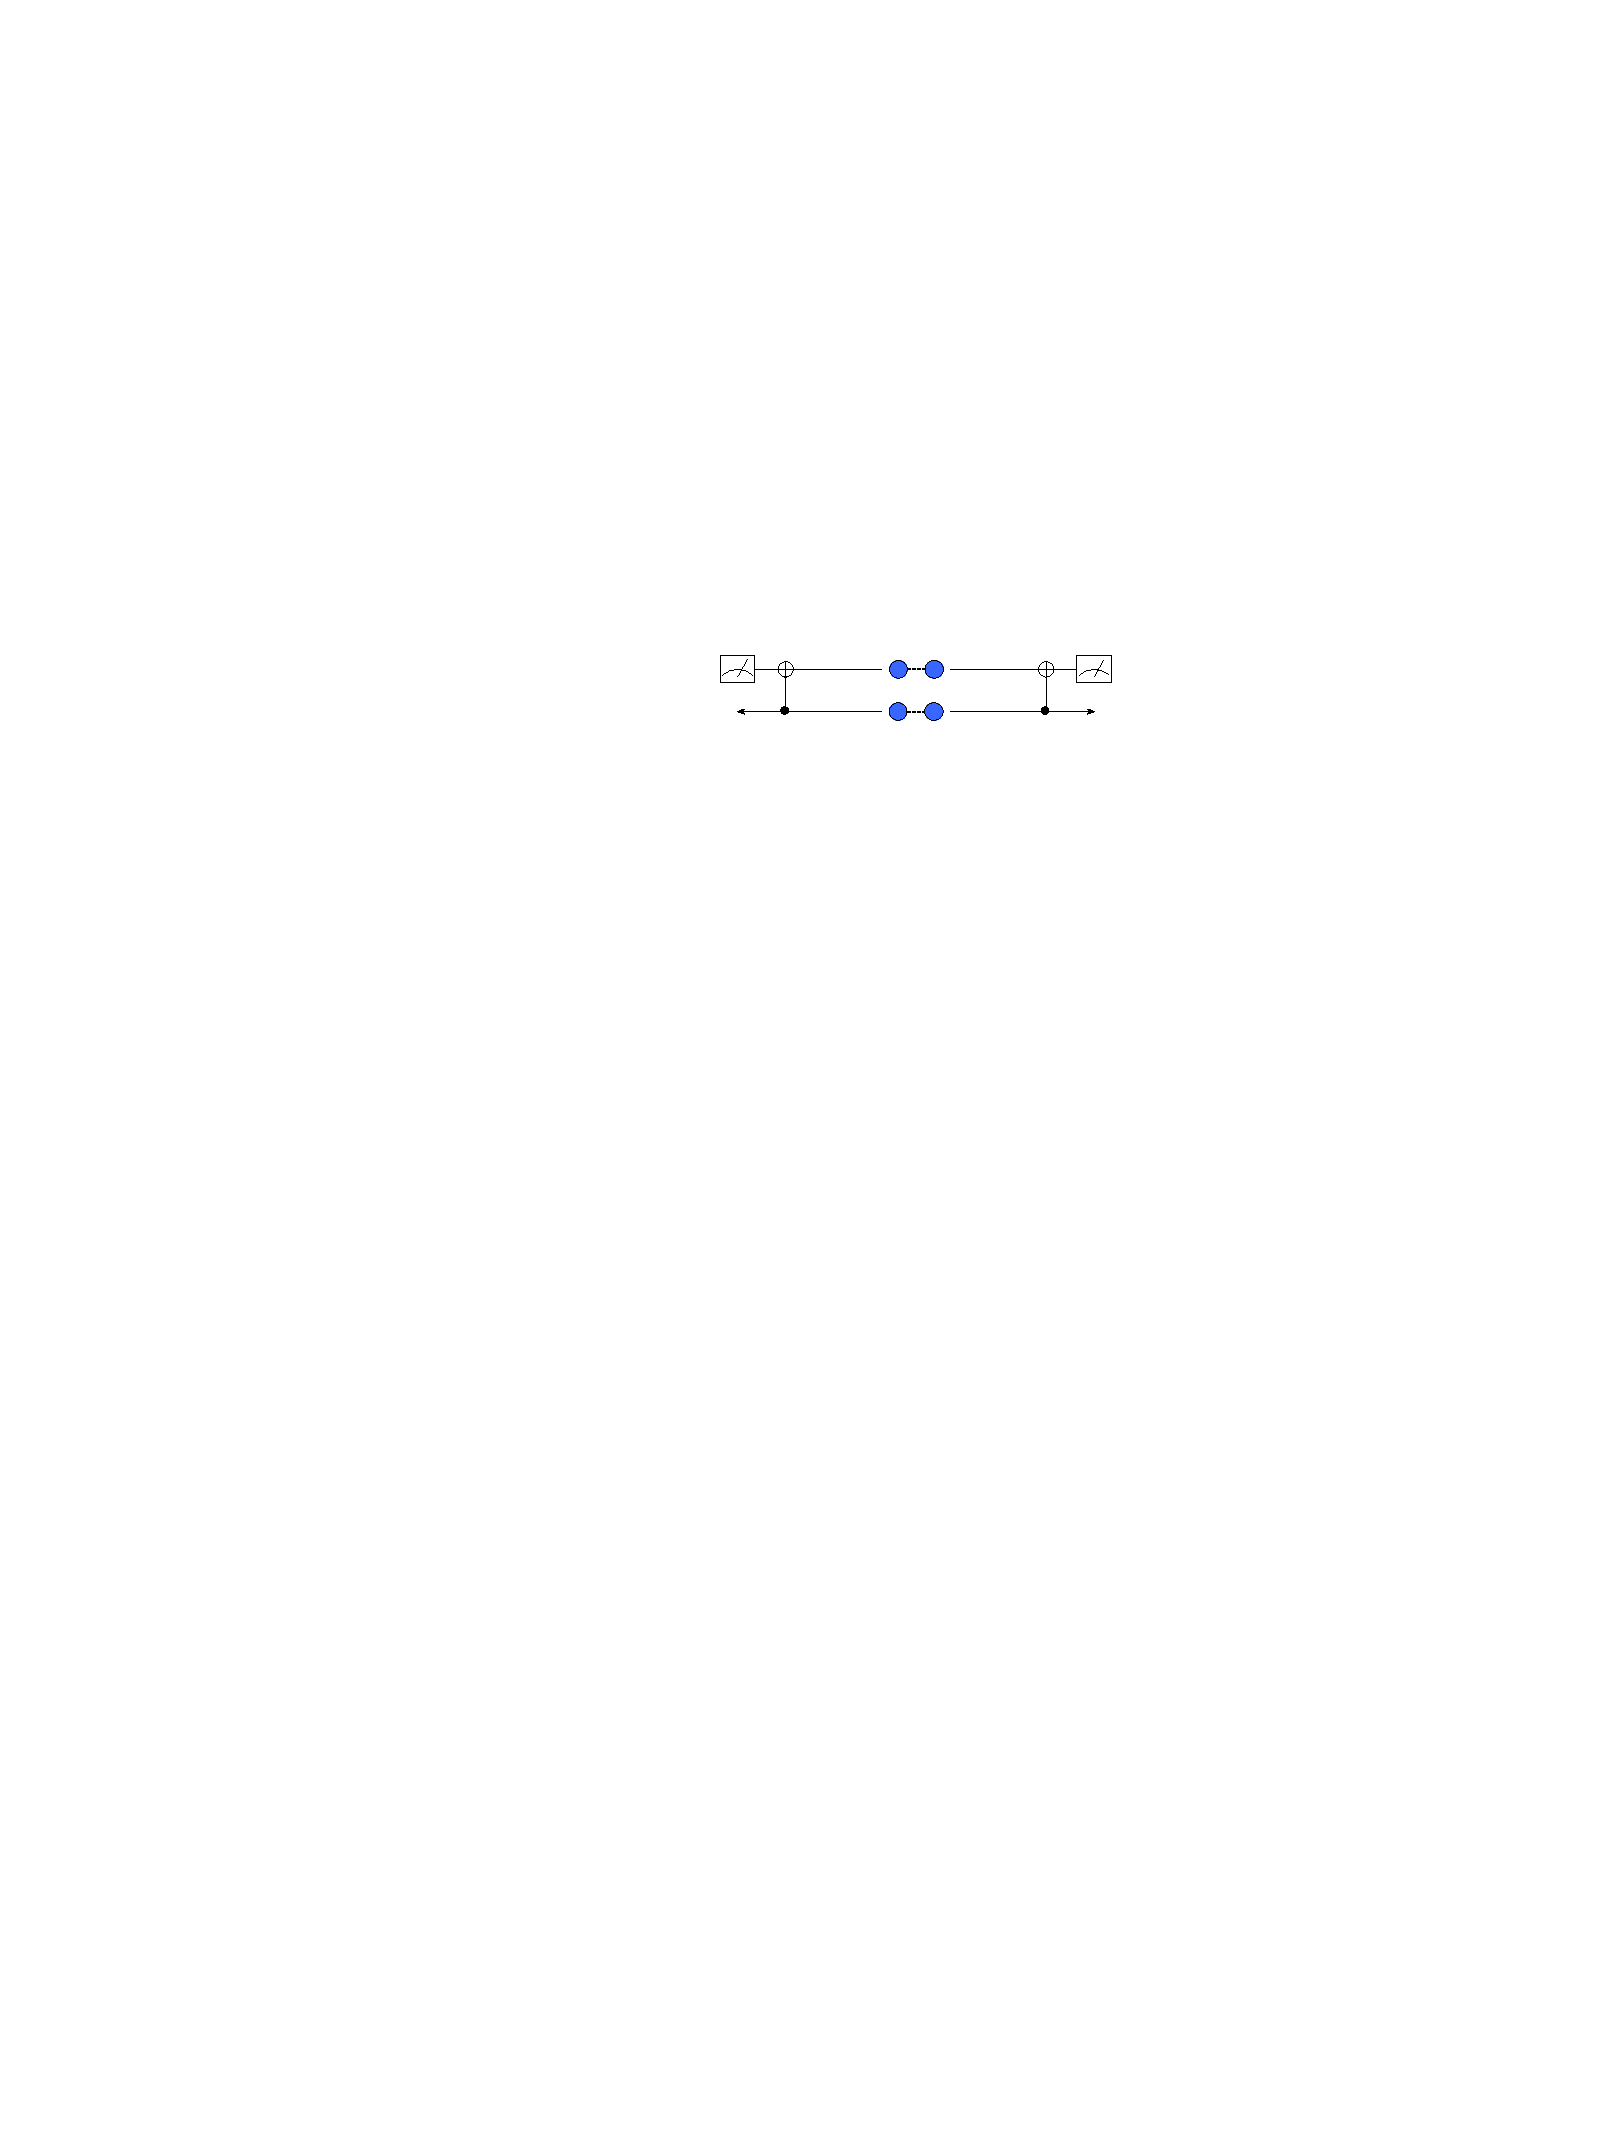
\includegraphics[clip=true, width=0.39\textwidth]{entanglement_purification}
\captionspacefig \caption{Protocol for entanglement purification of two noisy Bell pairs (blue) into a single less noisy Bell pair. Not shown are trivial single-qubit local corrections that may need to be made, depending upon measurement outcomes.} \label{fig:ent_purif_circ}\index{Entanglement purification protocol}
\end{figure}

Let us illustrate the operation of the circuit by example of different possible input states.

Suppose there were no errors, the ideal case. Then the input state was,
\begin{align}
\ket\psi_\mathrm{in} &= \ket{\Phi^+}_{1,2} \ket{\Phi^+}_{3,4}\\
&= \frac{1}{2}(\ket{0}_1\ket{0}_2+\ket{1}_1\ket{1}_2)(\ket{0}_3\ket{0}_4+\ket{1}_3\ket{1}_4).\nonumber
\end{align}
Upon parity measurement we obtain,
\begin{align}
\hat\Pi^+_{1,3} \ket{\Phi^+}_{1,2}\ket{\Phi^+}_{3,4} &= \ket{\Phi^+}_{2,4},\nonumber \\
\hat\Pi^-_{1,3} \ket{\Phi^+}_{1,2}\ket{\Phi^+}_{3,4} &= \hat{X}_2\ket{\Phi^+}_{2,4},
\end{align}
and we obtain the desired output Bell pair (with an $\hat{X}$ correction in the case of the odd-parity outcome).

Note that if both qubits from one Bell pair are subject to bit-flips, this is equivalent to no error, since,
\begin{align}
	\hat{X}_1\hat{X}_2\ket{\Phi^+}_{1,2}=\ket{\Phi^+}_{1,2}.
\end{align}

Now suppose there was a bit-flip error on the first qubit of the first pair. Now the input state is,
\begin{align}
\ket\psi_\mathrm{in} &= \hat{X}_1 \ket{\Phi^+}_{1,2} \ket{\Phi^+}_{3,4}\\
&= \frac{1}{2}(\ket{1}_1\ket{0}_2+\ket{0}_1\ket{1}_2)(\ket{0}_3\ket{0}_4+\ket{1}_3\ket{1}_4).\nonumber
\end{align}
Now upon parity measurement we obtain,
\begin{align}
\hat\Pi^+_{1,3} \hat{X}_1\ket{\Phi^+}_{1,2} \ket{\Phi^+}_{3,4} &= \hat{X}_2\ket{\Phi^+}_{2,4},\nonumber \\
\hat\Pi^-_{1,3} \hat{X}_1\ket{\Phi^+}_{1,2} \ket{\Phi^+}_{3,4} &= \ket{\Phi^+}_{2,4},
\end{align}
and following correction we achieve a bit-flipped Bell pair.

Finally, with both Bell pairs subject to a single bit-flip,
\begin{align}
\ket\psi_\mathrm{in} &= \hat{X}_1\hat{X}_3 \ket{\Phi^+}_{1,2}\ket{\Phi^+}_{3,4} \\
&= \frac{1}{2}(\ket{1}_1\ket{0}_2+\ket{0}_1\ket{1}_2)(\ket{1}_3\ket{0}_4+\ket{0}_3\ket{1}_4).\nonumber
\end{align}
Upon performing the parity measurement,
\begin{align}
\hat\Pi^+_{1,3} \hat{X}_1\hat{X}_3\ket{\Phi^+}_{1,2} \ket{\Phi^+}_{3,4} &= \ket{\Phi^+}_{2,4},\nonumber \\
\hat\Pi^-_{1,3} \hat{X}_1\hat{X}_3\ket{\Phi^+}_{1,2} \ket{\Phi^+}_{3,4} &= \hat{X}_2\ket{\Phi^+}_{2,4},
\end{align}
recovering the expected Bell pair, without an erroneous bit-flip.

Evidently, the output Bell pair is subject to an unexpected bit-flip iff one of the Bell pairs was subject to a bit-flip error. This yields the output fidelity,
\begin{align}
F_\mathrm{out} = \frac{{F_\mathrm{in}}^2}{{F_\mathrm{in}}^2 + (1-F_\mathrm{in})^2},
\end{align}
and thus the purification protocol improves fidelity provided that \mbox{$F_\mathrm{out}>F_\mathrm{in}$}, which implies the input fidelity must satisfy \mbox{$F_\mathrm{in}>1/2$}.

%
% 3-Qubit Code
%

\subsection{3-qubit code}\index{3-qubit code}

The first described QEC\index{Quantum error correction (QEC)} code was the 3-qubit code\index{3-qubit code} (or redundancy code) by \cite{bib:Shor95} for redundantly encoding a single logical qubit into three encoded qubits, allowing the detection and correction of at most a single bit-flip error between the encoded qubits. Measurement of the three ancillary qubits yields a \textit{syndrome}\index{Syndrome}, which identifies where the error took place, allowing it to be subsequently corrected with feedforward. This protocol is shown in Alg.~\ref{alg:three_QEC}.

By switching into a Hadamard-rotated basis, the same code could equivalently correct against at most a single phase-flip error (since \mbox{$\hat{H}\hat{X}\hat{H}=\hat{Z}$}).

\begin{table}[!htbp]
\begin{mdframed}[innertopmargin=3pt, innerbottommargin=3pt, nobreak]
\texttt{
function ThreeQubitCode($\ket\psi$):
\begin{enumerate}
\item Using two CNOT gates, redundantly encode the logical single-qubit state,
\begin{align}
\ket\psi=\alpha\ket{0}+\beta\ket{1},
\end{align}
into the 3-qubit state,
\begin{align}
\ket\psi_R &= \hat{\mathrm{CNOT}}_{1,2}\hat{\mathrm{CNOT}}_{1,3}\ket\psi\ket{00} \nonumber \\
&= \alpha\ket{000}+\beta\ket{111}.
\end{align}
\item Independently apply bit-flip channels $\mathcal{E}_X$ to each of the three encoded qubits.
\item If exactly one bit-flip operation was applied in total, the three possible erroneous encoded states are,
\begin{align}
\ket\psi_1 &= \hat{X}_1 \ket\psi_R = \alpha\ket{001}+\beta\ket{110}, \nonumber \\
\ket\psi_2 &= \hat{X}_2 \ket\psi_R = \alpha\ket{010}+\beta\ket{101}, \nonumber \\
\ket\psi_3 &= \hat{X}_3 \ket\psi_R = \alpha\ket{100}+\beta\ket{011}.
\end{align}
\item Determine the parity of each of the three pairs of encoded qubits.
\item Assuming at most a single bit-flip operation has occurred on the encoded state, the three parity outcomes uniquely determine which encoded qubit the bit-flip was applied to.
\item Apply classically-controlled bit-flip recovery operations, $\mathcal{R}$, to correct the encoded state, recovering $\ket\psi_R$.
\item Apply the inverse of the encoding operation to recover $\ket\psi$.
\item $\Box$
\end{enumerate}}
\begin{align}
\Qcircuit @C=1.3em @R=.6em {
  & \lstick{\ket{\psi}} & \ctrl{2} & \gate{\mathcal{E}_X}  & \qw & \qw              & \ctrl{3}  & \qw       & \ctrl{4} & \qw & \multigate{2}{\ \mathcal{R}\ } & \qw \\
  & \lstick{\ket{0}}    & \targ    & \gate{\mathcal{E}_X}  & \qw & \qw              & \ctrl{2}  & \ctrl{2}  & \qw      & \qw & \ghost{\ \mathcal{R}\ } \qw & \qw \\
  & \lstick{\ket{0}}    & \targ    & \gate{\mathcal{E}_X}  & \qw & \qw              & \qw       & \ctrl{2}  & \ctrl{3} & \qw & \ghost{\ \mathcal{R}\ } \qw & \qw \\
  &          &          &          & & \lstick{\ket{0}} & \targ \qw & \qw       & \qw      & \meter & \control \cw \cwx \\
  &          &          &          & & \lstick{\ket{0}} & \qw       & \targ \qw & \qw      & \meter & \control \cw \cwx \\
  &          &          &          & & \lstick{\ket{0}} & \qw       & \qw       & \targ    & \meter & \control \cw \cwx
} \nonumber
\end{align}
\end{mdframed}
\captionspacealg \caption{3-qubit code for protecting against at most a single logical bit-flip error. The doubly-controlled CNOT gates represent parity measurements, \mbox{$n_3=n_1\oplus n_2$}, where $n_i$ represents the value of the $i$th qubit. In a Hadamard-rotated basis, the same circuit may be employed to protect against a single phase-flip error. And by concatenating the two we obtain a 9-qubit code protecting against a single depolarising error (i.e joint bit-flip/phase-flip), which is a universal single-qubit error model.} \label{alg:three_QEC}
\end{table}

%
% 9-Qubit Code
%

\subsection{9-qubit code}\index{9-qubit code}

By taking two instances of the 3-qubit code, one implementing bit-flip correction and the other implementing phase-flip correction, and concatenating them, we can define a 9-qubit code, which protects against at most a single bit-flip and a single phase-flip. Joint protection against both the bit-flip and phase-flip operators ($\hat{X}$ and $\hat{Z}$) in turn allows error correction against a single depolarising error, the most general type of logical error, which completely destroys a single qubit.

This is the simplest construction of a code which protects against a single depolarising event. But it is not the most efficient, and numerous more resource-savvy codes for protecting against Pauli errors exist, such as Steane's 7-qubit code\index{Steane code} \cite{SteaneCode}.

%
% Stabiliser Codes
%

\subsection{Stabiliser codes}\index{Stabiliser codes}\label{sec:stab_code}

\comment{To do}

%
% Surface Codes
%

\subsection{Surface codes}\index{Surface codes}

\comment{Discuss genus and how this adds logical qubits.}

If the intention is to perform quantum computations using cluster states shared over a network, QEC and fault-tolerance \textit{must} be taken into consideration, or catastrophic algorithmic failure will inevitably follow -- the cluster state model is no different from the circuit model in this respect. Fault-tolerance theory places hard thresholds on the amount of noise (typically depolarising errors and loss) qubits may be subject to in order for fault-tolerance to be possible and computations to succeed. This places strict QoS (Sec.~\ref{sec:QOS}) constraints on the network, which can be accommodated for using the usual depolarising and efficiency cost metrics when developing networking strategies and link performance requirements.

It has been shown that fault-tolerance is possible within the cluster state model \cite{bib:NielsenDawson04, bib:Dawson06} using variations of conventional QEC codes. However, more importantly, from cluster states certain \textit{topological QEC codes} \cite{???} can be readily constructed. This implements a form of QEC-encoded measurement-based quantum computing protocol, where the computation proceeds in a measurement-based fashion, but is `natively' fault-tolerant.

These codes have been shown to have very favourable fault-tolerance thresholds in terms of both depolarising noise and loss \cite{bib:StaceBarrettDohertyLoss, bib:BarrettStaceFT}, as well as frugal resource overhead compared to traditional concatenated codes. Additionally, loss- and gate-failure-tolerant codes, uniquely applicable to the cluster state model, have been described, with very favourable loss thresholds \cite{bib:Varnava05, bib:RalphHayes05, bib:Duan05}. 

Importantly, topological codes do not require joint measurements across the entire graph state, instead requiring only operations localised to small regions within the graph. Thanks to this, computation using such topological codes can remain distributed\index{Distributed quantum computation} without requiring the entire state to be held locally by a particular host, or requiring full access to the entire state by any particular user. As with cluster states, a large graph can be stitched together from a patchwork of smaller neighbouring graphs.

The most common topological code, which we will use here as an example, is the toric code\index{Toric code}, which resides on a lattice graph over the surface of a torus\footnote{As with cluster states, this graph needn't (but could) correspond to a network graph.}. As with cluster states (Sec.~\ref{sec:CSQC}), the toric code is most easily visualised in the stabiliser formalism\index{Stabiliser formalism}, and the toric code is an example of a stabiliser code\index{Stabiliser codes} (Sec.~\ref{sec:stab_code}). Consider a rectangular sub-graph of the torus. We place a qubit on each edge (not vertex) of the graph. Now we define two sets of stabiliser operators: \textit{star} ($\hat{S}_+$) and \textit{plaquette} ($\hat{S}_\square$) operators,
\begin{align} \index{Surface code stabilisers}\index{Star operator}\index{Plaquette operator}
	\hat{S}_+(v) &= \prod_{i\in e(v)} \hat{X}_i, \nonumber \\
	\hat{S}_\square(p) &= \prod_{i\in e(p)} \hat{Z}_i,
\end{align}
where $e(v)$ are the edges neighbouring vertex $v$, and $e(p)$ are the edges surrounding plaquette $p$. By definition, the toric code state, $\ket\psi_\mathrm{toric}$, satisfies the stabiliser relations,
\begin{align}
	\hat{S}_+(v) \ket\psi_\mathrm{toric} &= \ket\psi_\mathrm{toric} \,\forall\, v, \nonumber \\
	\hat{S}_\square(p) \ket\psi_\mathrm{toric} &= \ket\psi_\mathrm{toric} \,\forall\, p.
\end{align}
The stabilisers can be visualised graphically as per Fig.~\ref{fig:toric_code}.

\if 2\pubmode
	\begin{figure}[!htbp]
		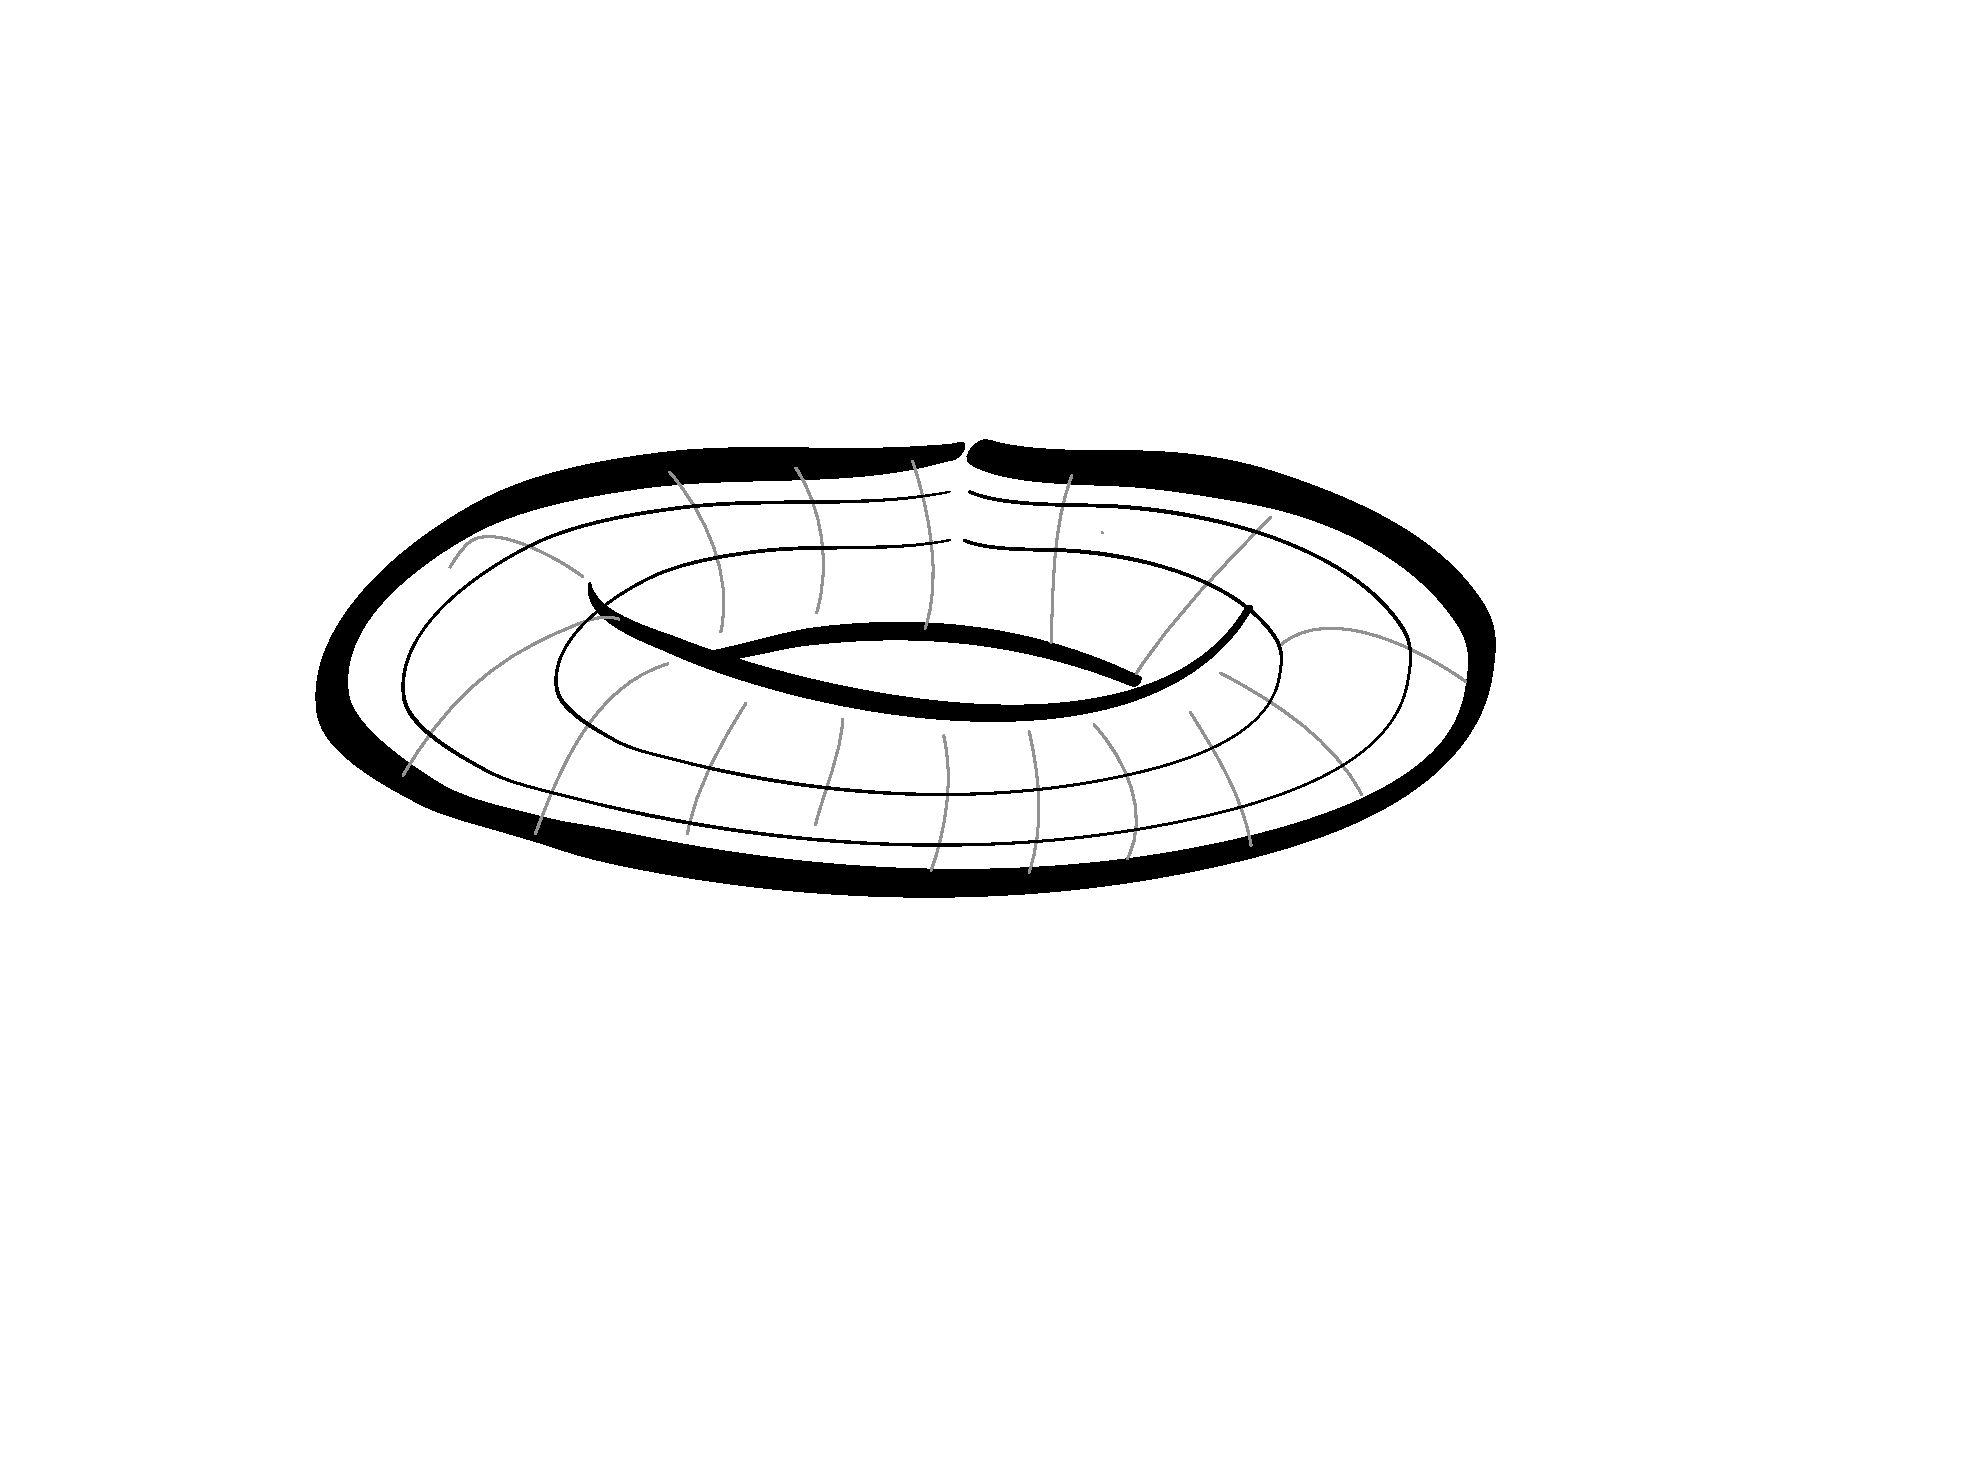
\includegraphics[clip=true, width=0.475\textwidth]{torus}\\
		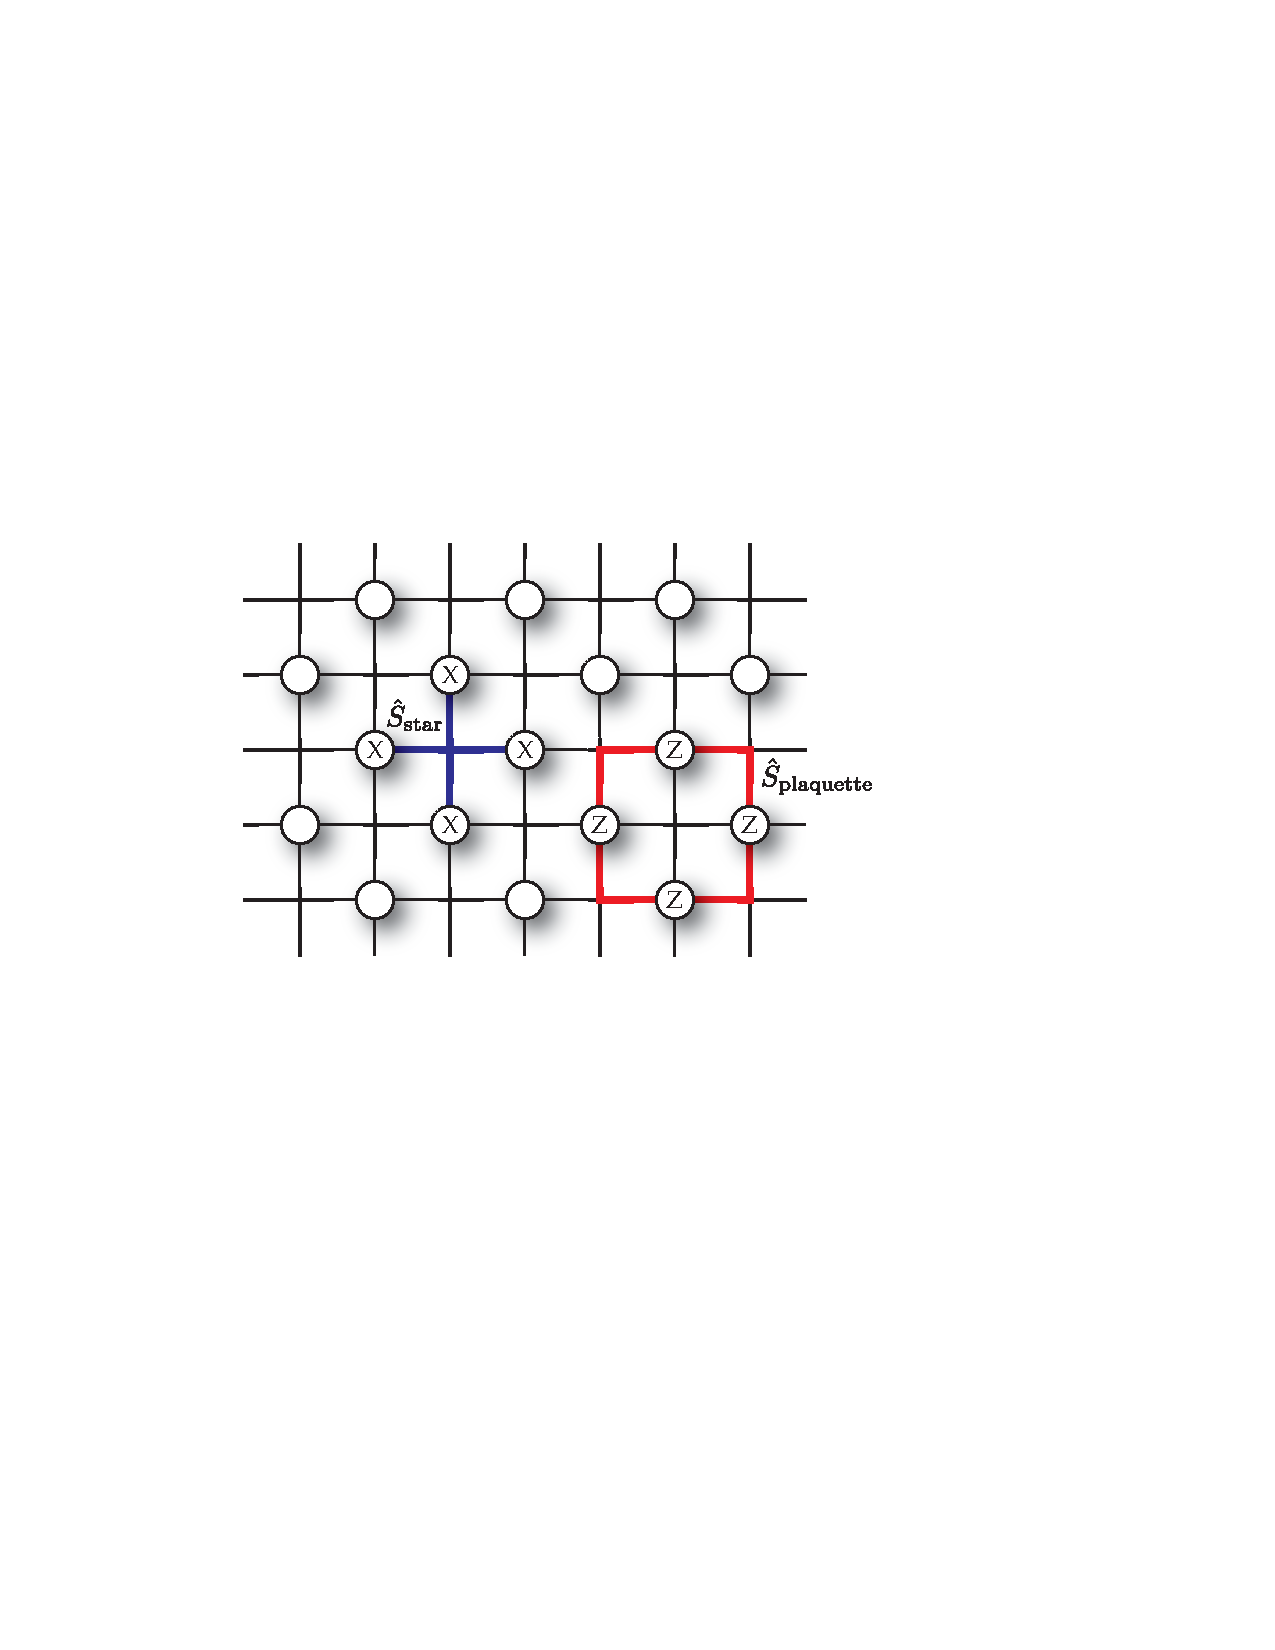
\includegraphics[clip=true, width=0.475\textwidth]{toric_code}
		\captionspacefig \caption{Graph representation of the toric QEC code, and its associated stabilisers. The graph resides on a torus (top), while the physical qubits reside on the embedded lattice (bottom). The star and plaquette stabilisers across all vertices, jointly specify the state of the graph up to two missing degrees of freedom, which encode a single logical qubit. Thus, a logical qubit is encoded jointly across the entire graph, not at any specific vertex. Logical operations are performed via operations following topological paths through the lattice (not shown). The graph may be distributed across multiple hosts for distributed quantum computation.} \label{fig:toric_code}
	\end{figure}
\else
	\begin{figure*}[!htbp]
		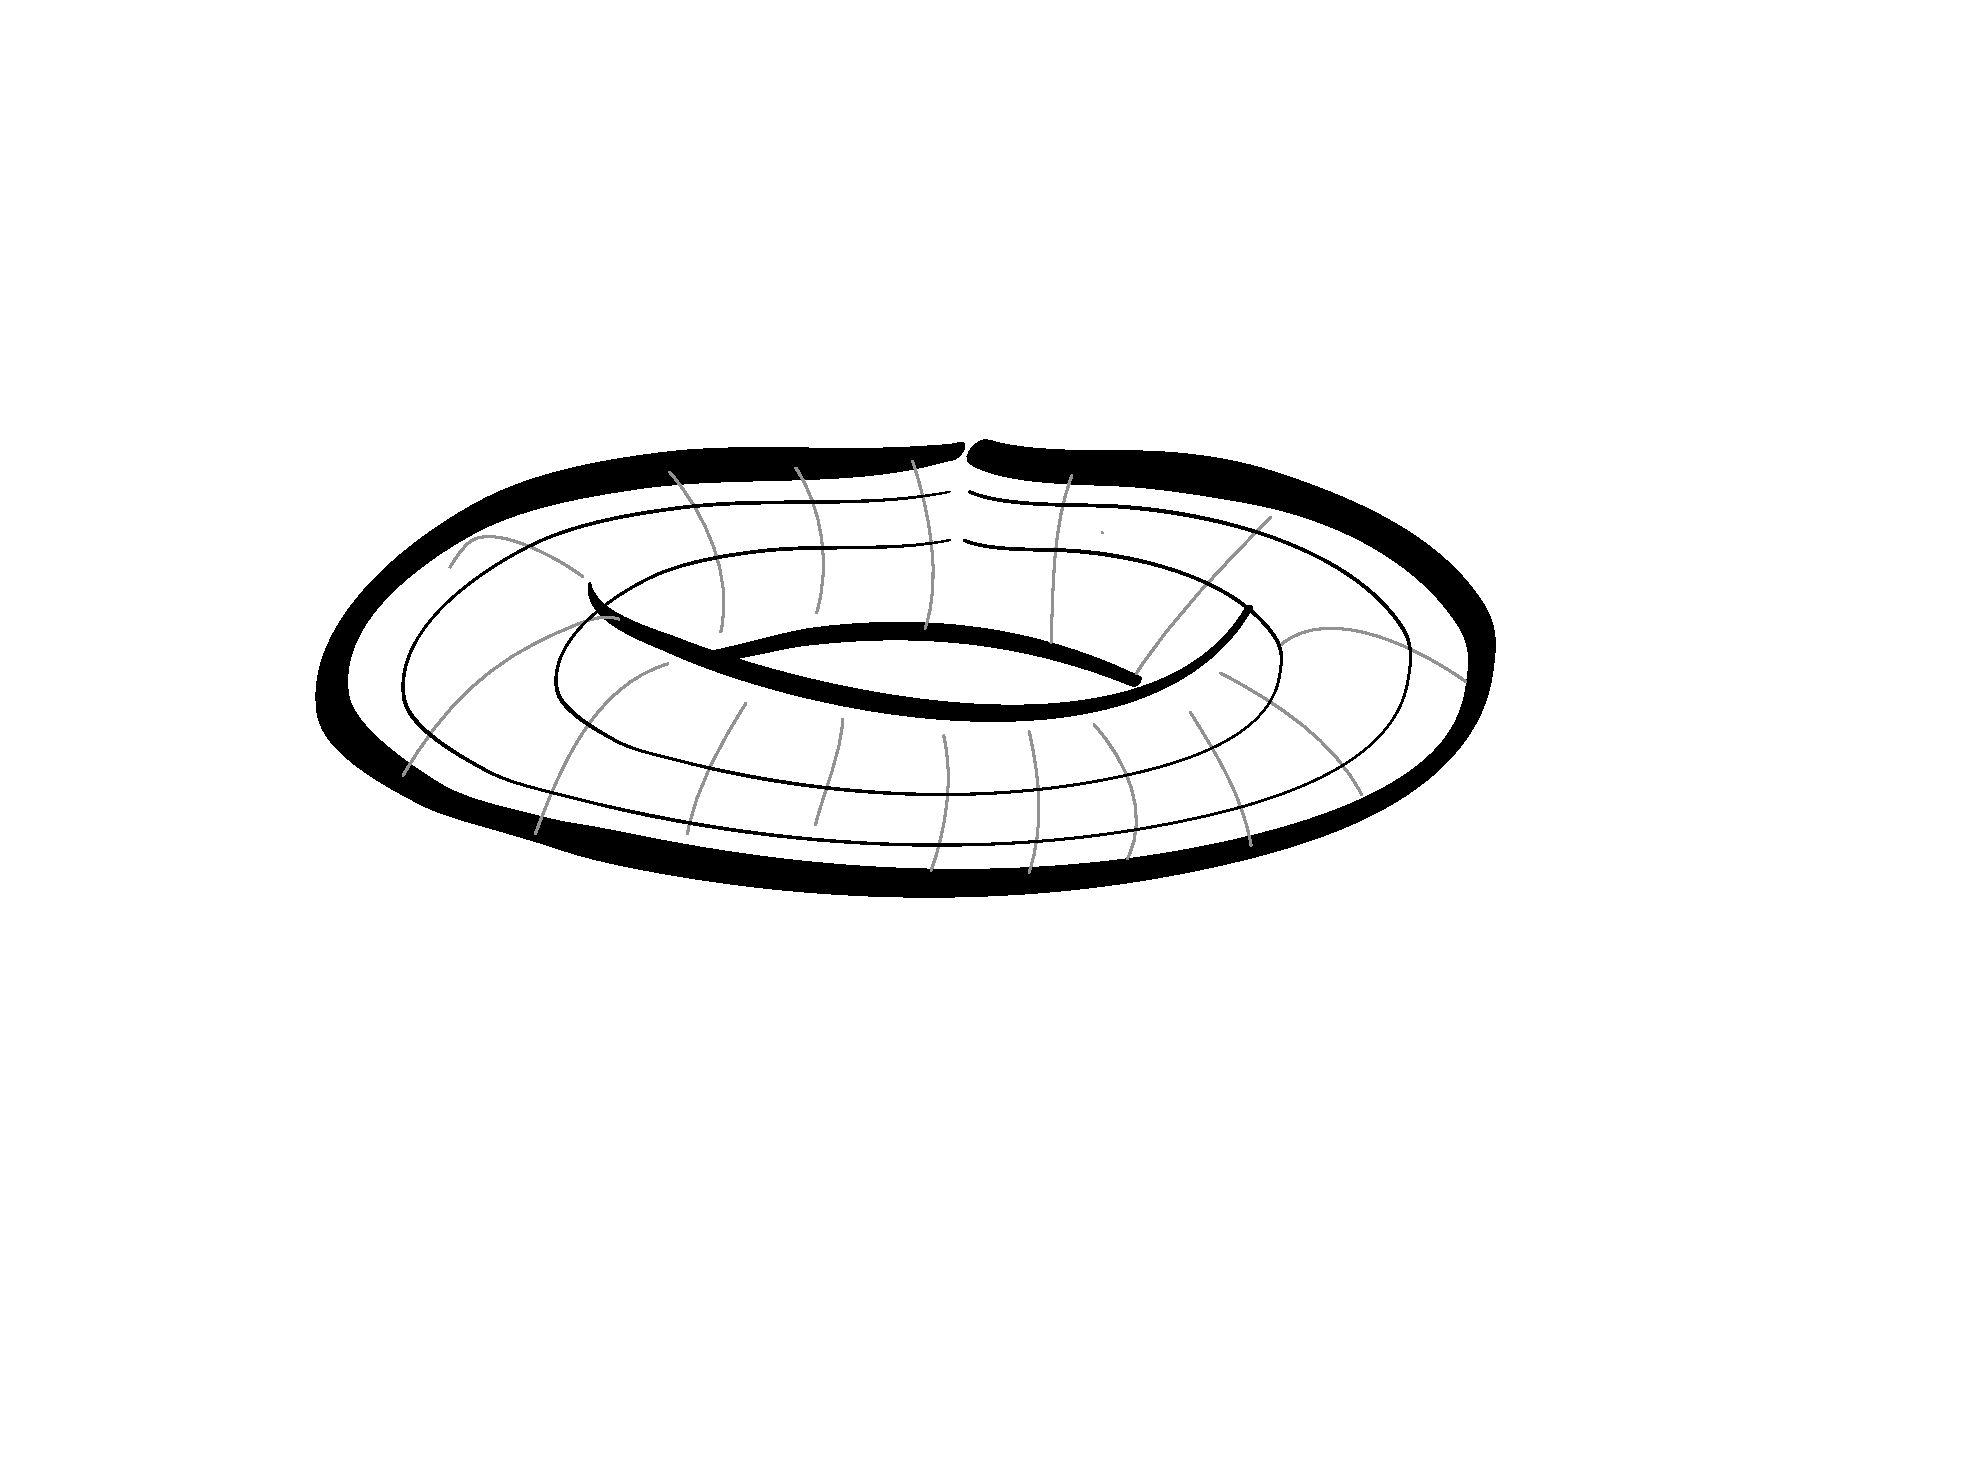
\includegraphics[clip=true, width=0.475\textwidth]{torus}
		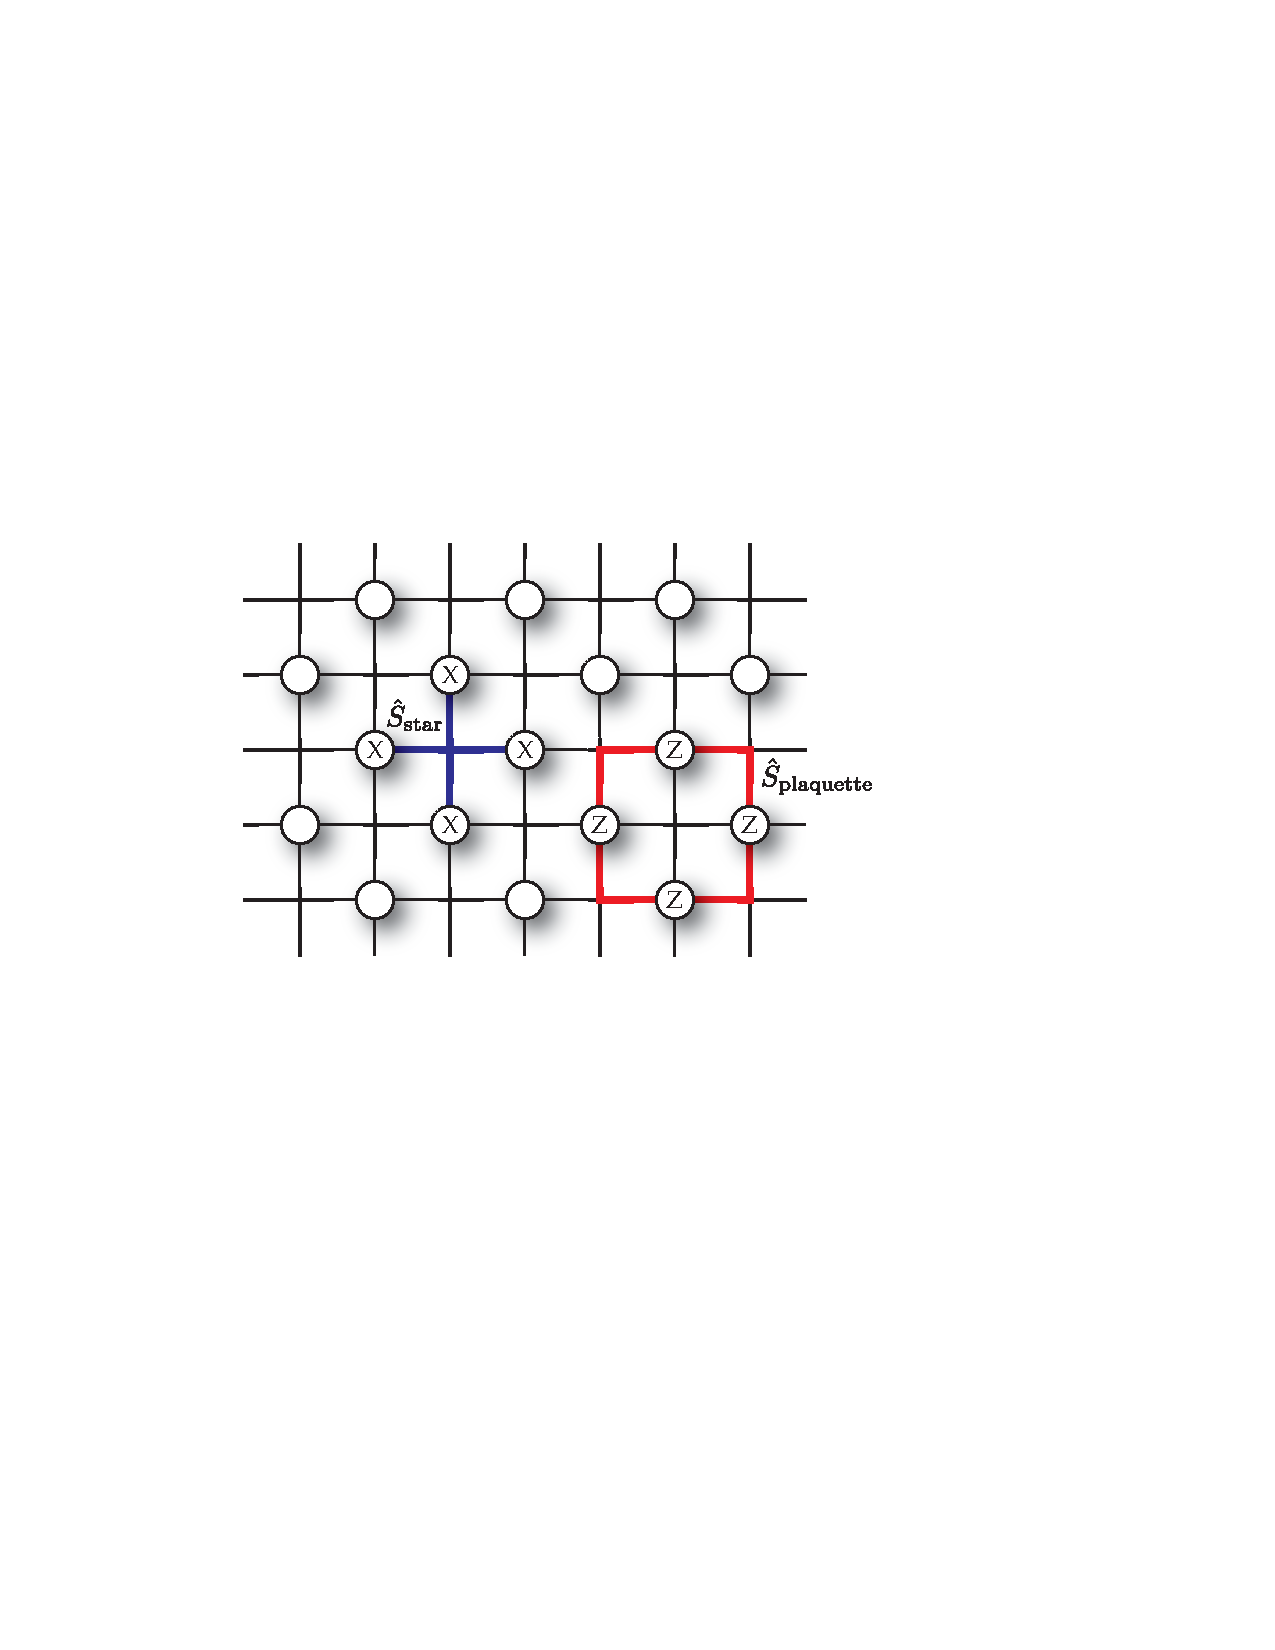
\includegraphics[clip=true, width=0.475\textwidth]{toric_code}
		\captionspacefig \caption{Graph representation of the toric QEC code, and its associated stabilisers. The graph resides on a torus (left), while the physical qubits reside on the embedded lattice (right). The star and plaquette stabilisers across all vertices, jointly specify the state of the graph up to two missing degrees of freedom, which encode a single logical qubit. Thus, a logical qubit is encoded jointly across the entire graph, not at any specific vertex. Logical operations are performed via operations following topological paths through the lattice (not shown). The graph may be distributed across multiple hosts for distributed quantum computation.} \label{fig:toric_code}
	\end{figure*}
\fi

Unlike the cluster state stabilisers from Eq.~(\ref{eq:CS_stab}), these stabilisers are insufficient to fully characterise a unique quantum state. Rather, there are two unspecified degrees of freedom, which allows for a single qubit to be represented. Modifications of the topology, in the form of holes in the lattice (the genus of the topology), allow larger numbers of qubits to be encoded. Logical operations are implemented by performing sequences of local gates and measurements across topologies over the surface.

The important feature to note is that logical qubits encoded into the toric code do not reside locally at any of the physical qubits in the topology. Rather, they reside jointly across the entire graph, which, like cluster states, might be partitioned across multiple hosts, enabling distributed computation.

Having defined the toric code as such, QEC proceeds in a similar manner to any other stabiliser code -- we measure all the stabilisers, yielding a syndrome\index{Error syndrome}, from which we can determine geometrically where errors took place in the graph, which can subsequently be corrected (if below threshold).

The simplest example of error detection is the scenario where a single bit-flip ($\hat{X})$ error has occurred in the graph. Now exactly two plaquette stabilisers (the ones upon which the respective qubit acts) will yield the $-1$ measurement outcome, instead of the expected $+1$ outcome. These two stabilisers will necessarily be neighbouring ones, overlapping at the qubit where the error took place. Thus, using this geometric reasoning, we are able to identify the location of the single $\hat{X}$ error and subsequently correct it. On the other hand, if there were too many errors, it is possible they could conspire against us to create ambiguity in the geometric argument for the location of the errors. The QEC procedure is illustrated in Fig.~\ref{fig:toric_code}.

\begin{figure}[!htbp]
	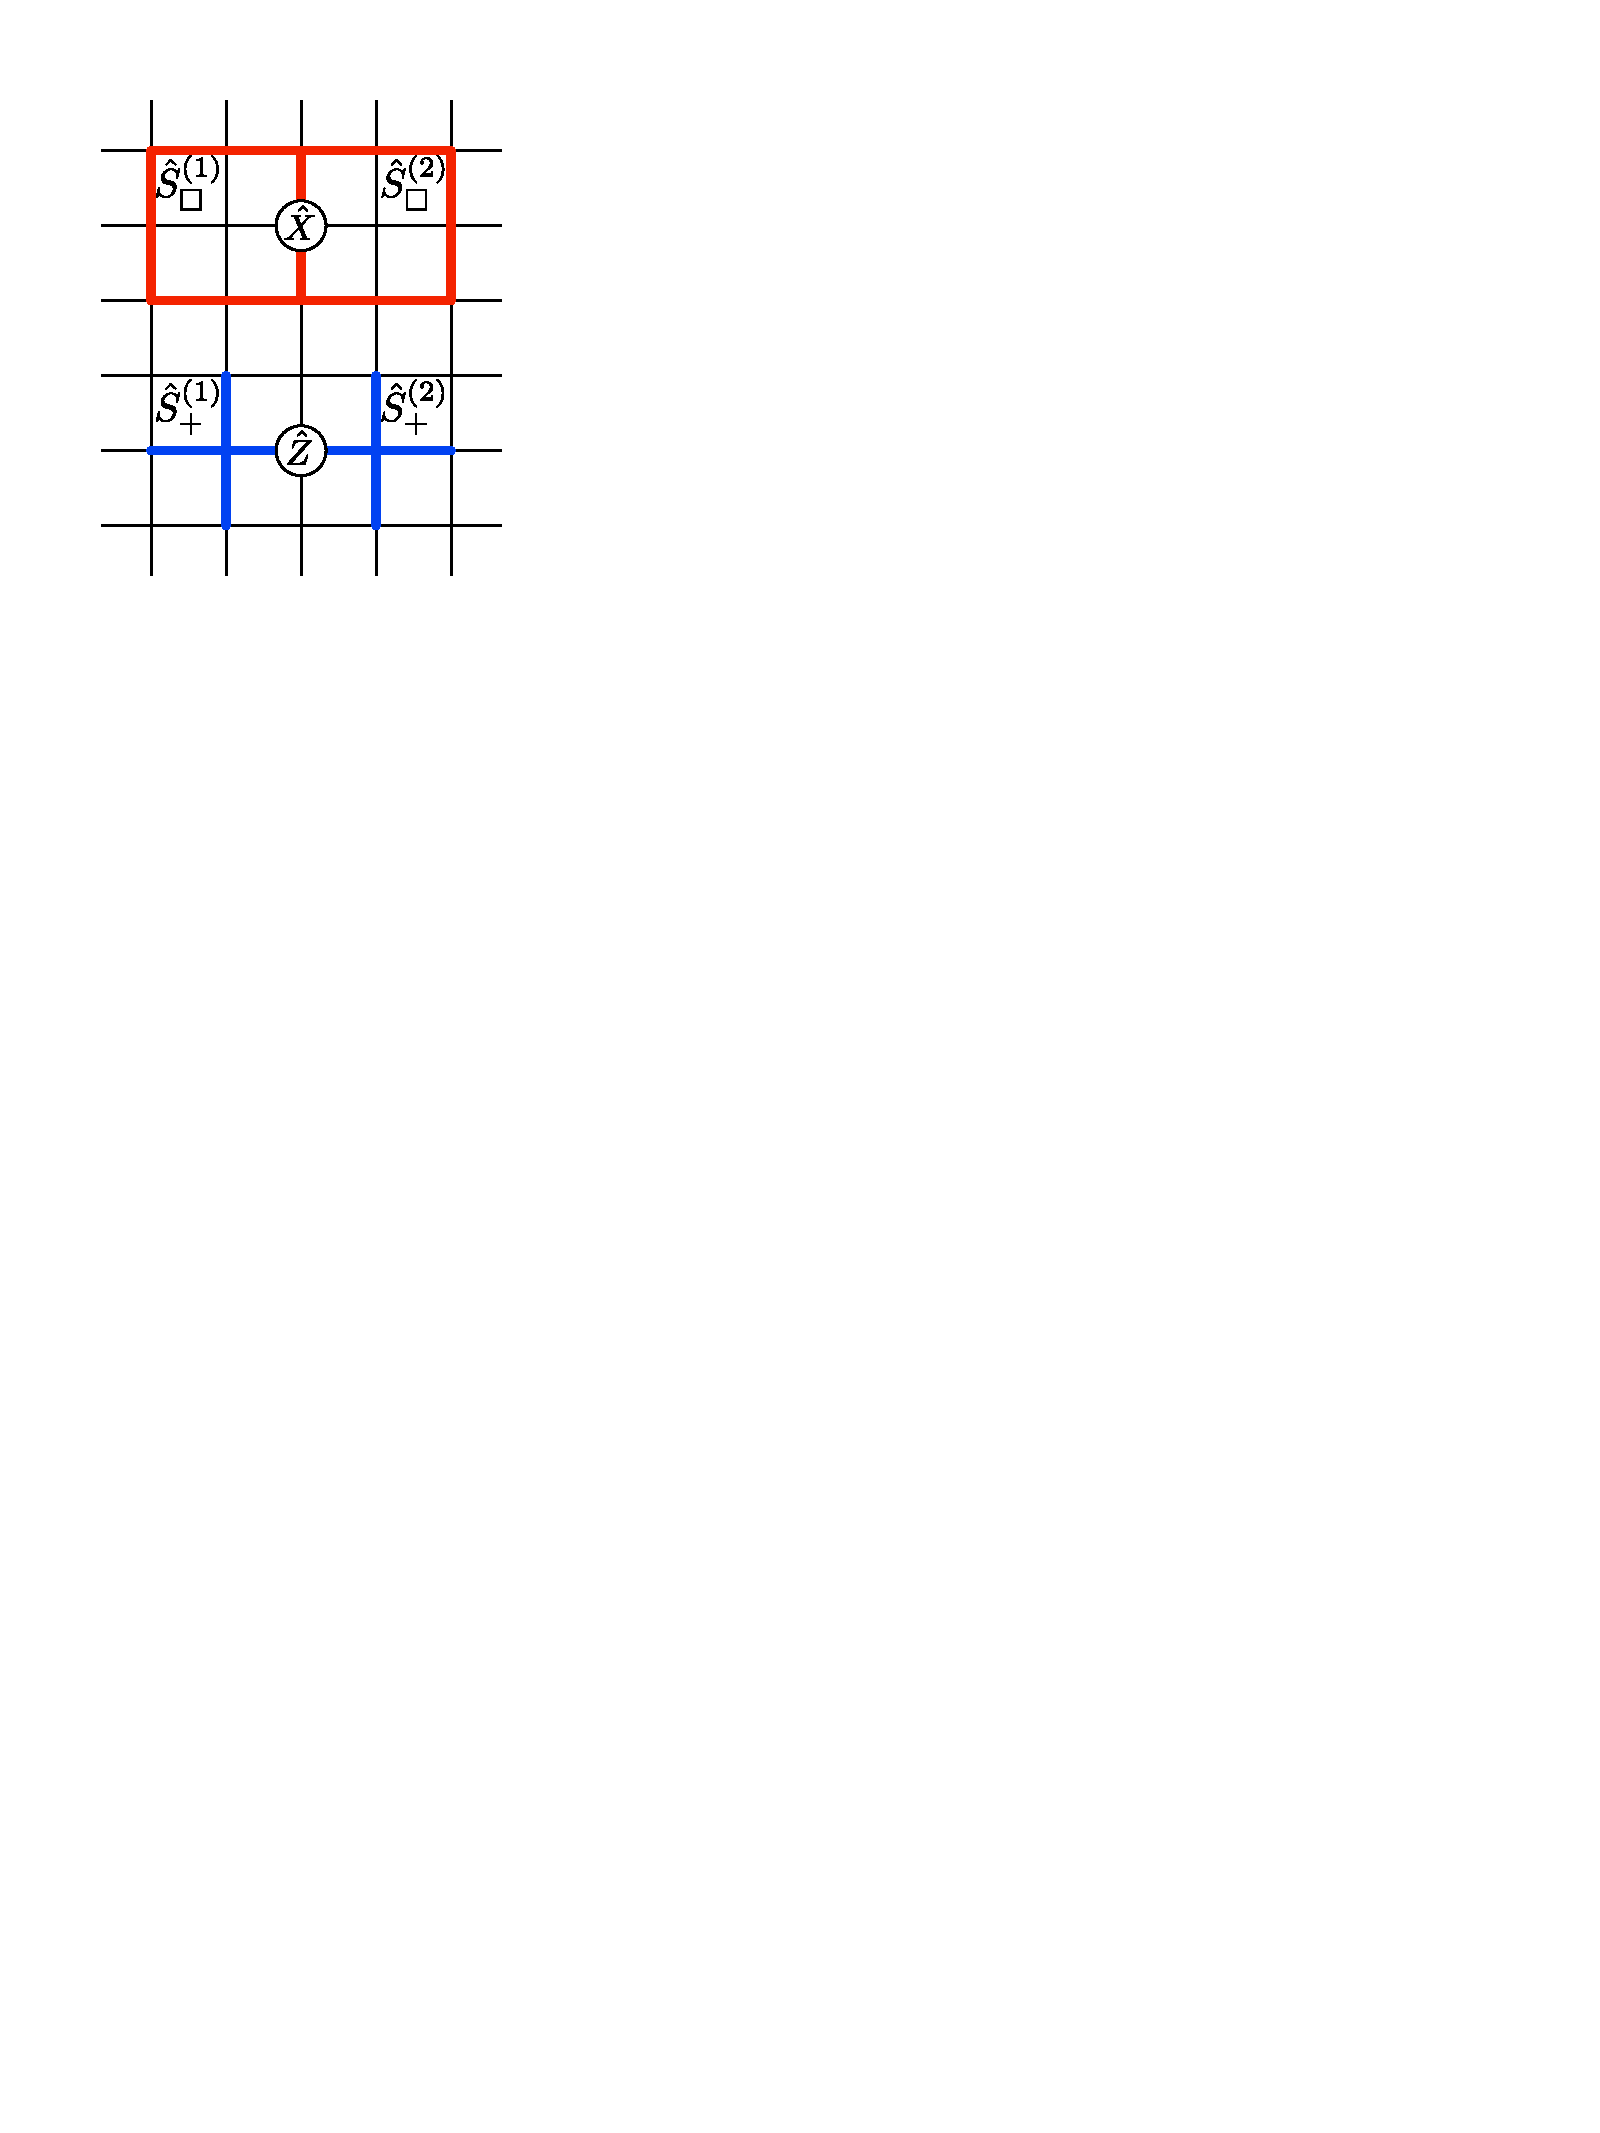
\includegraphics[clip=true, width=0.3\textwidth]{toric_code_correction}
	\captionspacefig \caption{QEC of a single bit-flip (top) and phase-flip (bottom) error via measuring two overlapping stabilisers. If there is at most one bit- or phase-flip error, as per this graphic, then upon measuring all the star and plaquette stabilisers, only those whose qubits are affected by the error channel will yield the $-1$ measurement outcome, the others all yielding $+1$. Such an error will affect exactly two stabilisers, whose qubit in common must have been the one affected by the respective error, which can subsequently be corrected since the type of the error and its location are known. Thus, in this example, all of the $\hat{S}_+^{(1)}$, $\hat{S}_+^{(2)}$, $\hat{S}_\square^{(1)}$ and $\hat{S}_\square^{(2)}$ stabilisers will yield $-1$ outcomes for the shown $\hat{X}$ and $\hat{Z}$ errors, whereas any of the remaining (not shown) $\hat{S}_k^{(j)}$ will yield $+1$ outcomes, which uniquely specifies where those errors took place.}\label{fig:toric_corr}	
\end{figure}

Importantly, the stabilisers are all defined over geometrically localised neighbourhood regions, and do not require long-range measurements, making this type of code suitable to distributed models for quantum computation, much like cluster states.

Logical operations similarly have geometric interpretations. Most simply, logical Pauli-$\hat{X}$ and -$\hat{Z}$ gates may be implemented by applying chains of local Pauli operations along topological paths, specifically closed loops around the two different axes of the torus (Fig.~\ref{fig:toric_code_paulis}. These topologies may be deformed, provided that they are topologically equivalent to the desired closed loops, hence the name `topological code'. With more qubits and more elaborate gates, similar topological definitions exist for implementing logical gates on encoded qubits.

\begin{figure}[!htbp]
	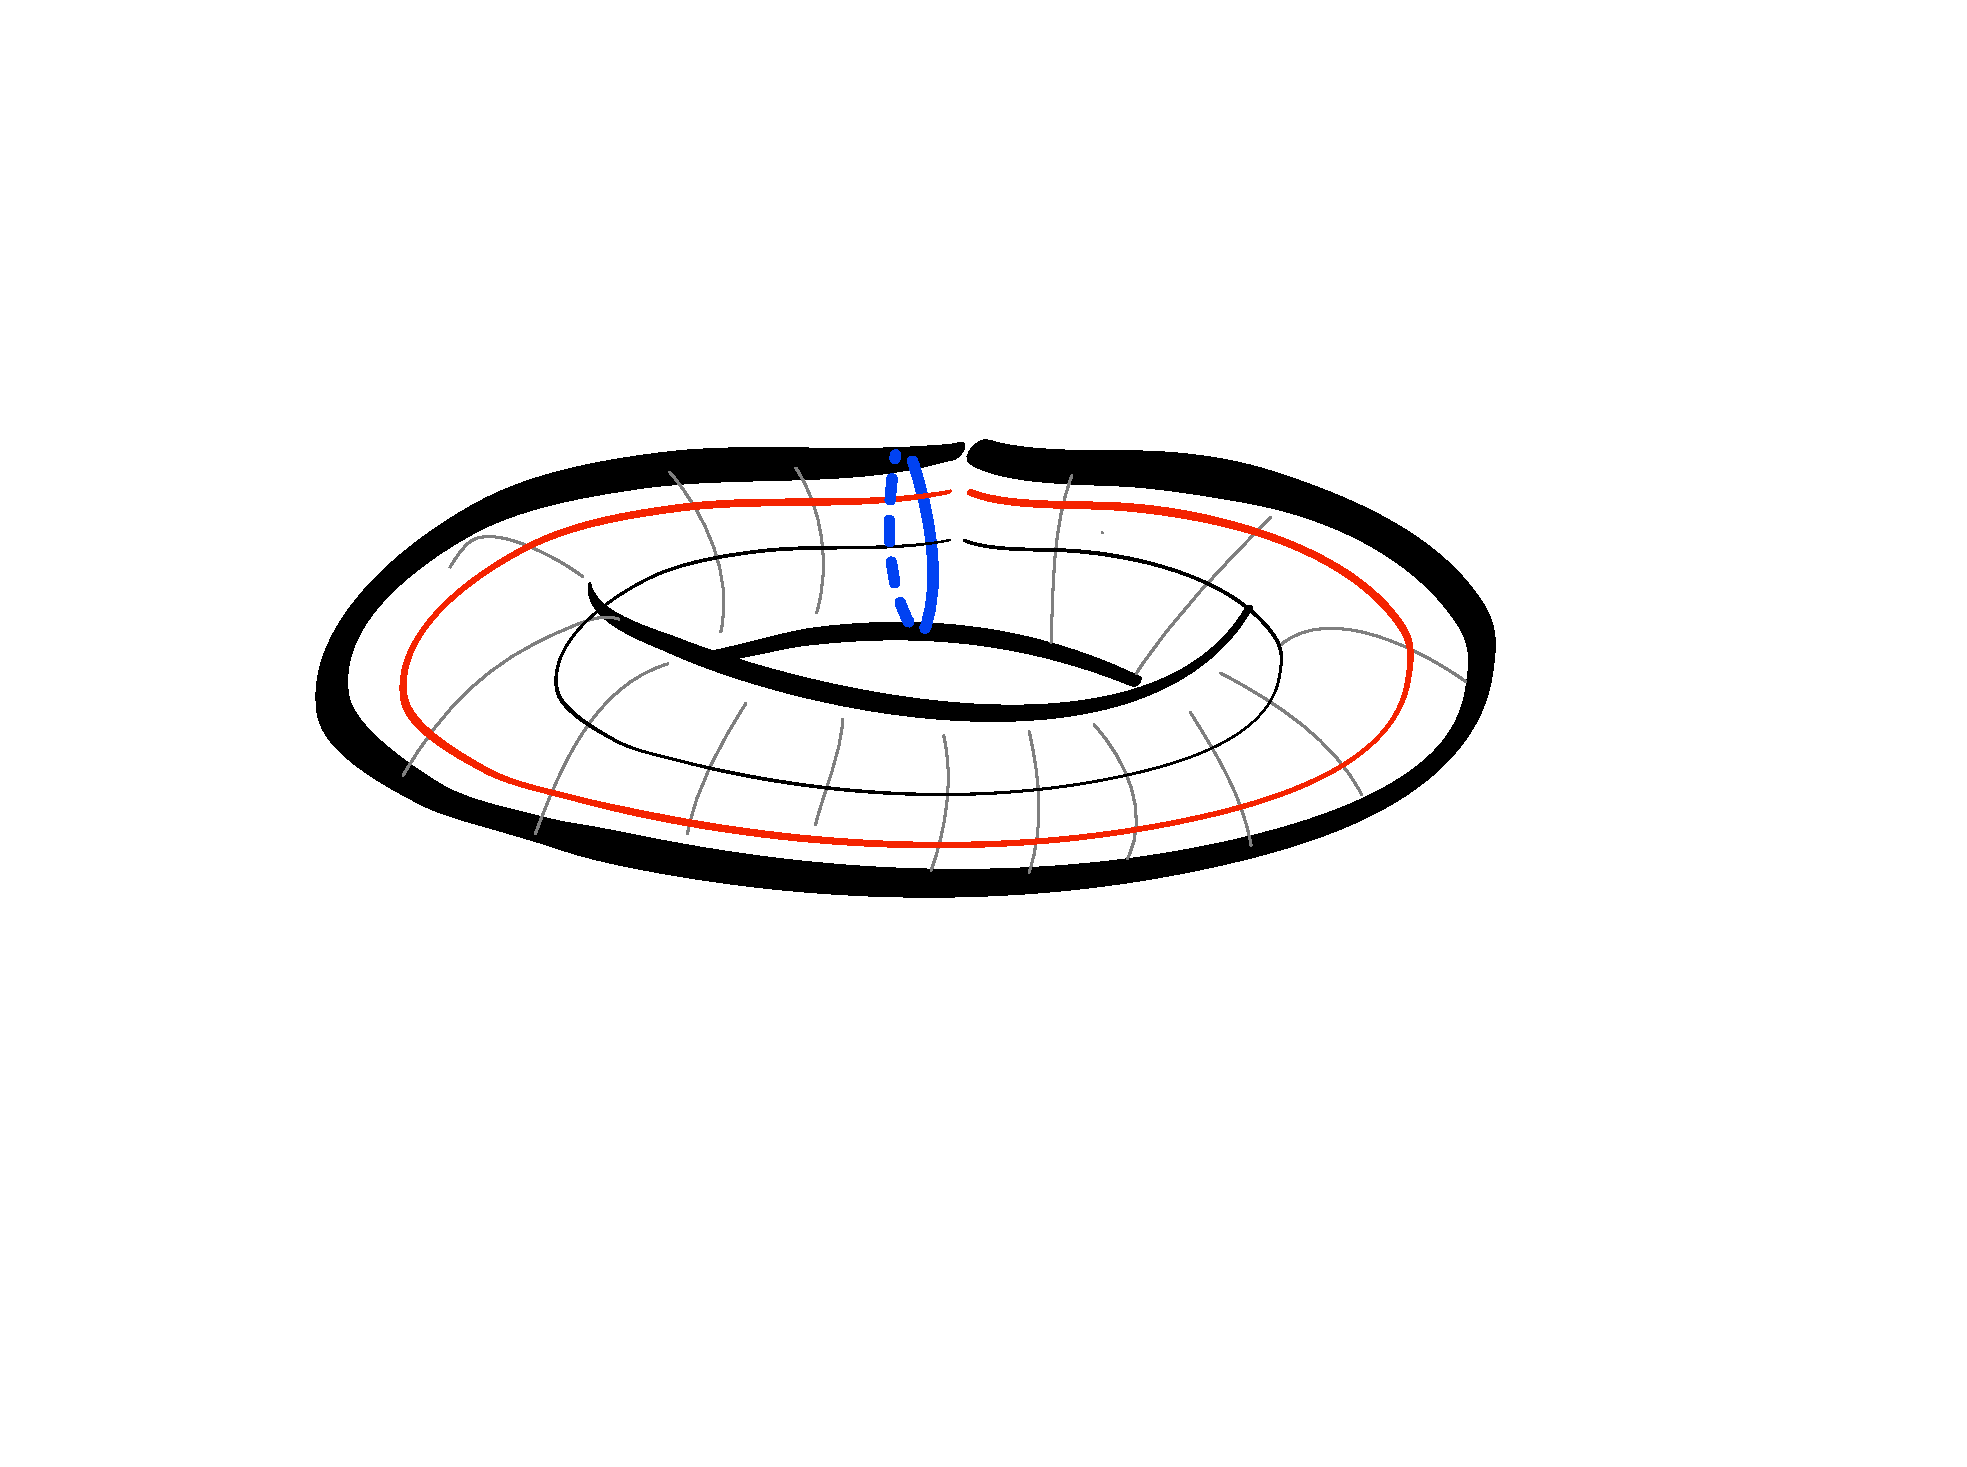
\includegraphics[clip=true, width=0.475\textwidth]{torus_paulis}
	\captionspacefig \caption{Implementation of logical Pauli-$\hat{X}$ (\comment{which colour?}) and -$\hat{Z}$ (\comment{which colour?}) operations on a toric code qubit via the application of a chain of local Paulis. The chains must circumnavigate the torus around either axis. Any path topologically equivalent to such a circumnavigation of the torus is sufficient, enabling paths to bypass defects in the lattice.} \label{fig:toric_code_paulis}
\end{figure}

\comment{What about the actual computation? Can this still be distributed when we do the topological gates etc?}

\comment{Figures for thresholds FT and QEC}

\comment{Explain stabiliser measurement and how this yields error syndromes}

\comment{Explain logical operations on code}

\comment{Explain how number of logical qubits can be increased by changing topology}

\comment{How to convert cluster states to topological codes, or any other way of preparing them. Add discussion of how to perform gates.}

\comment{Figure for both examples of this -- under and over threshold!}

\comment{Missing degree of freedom in stabilisers defines qubit. How does topology (genus) relate to number of logical qubits?}

%
% Unitary Error Averaging
%

\subsection{Unitary error averaging} \index{Quantum error correction (QEC)}\index{Unitary error averaging}\label{sec:error_averaging}

Aside from the \textit{active} QoS techniques discussed until now, there is also a recently described \textit{passive} technique that requires no feedforward to operate. This technique, called \textit{unitary error averaging} \cite{MarshmanLundRohde}, is formulated specifically in the linear optical context. It is an open question whether it generalises to other models, such as conventional quantum circuits.

Suppose we desire to implement some linear optics unitary network, $\hat{U}_\mathrm{target}$, but our fabrication techniques are imperfect and we instead implement a close approximation to it. How can we overcome this?

\cite{MarshmanLundRohdeRalph} showed that by using an optical fanout\index{Fanout operation} operation, which splits a set of optical modes equally across multiple sets of modes in a type of redundant encoding\footnote{The optical fanout operation effectively maps single-photon states to W-states (Sec.~\ref{sec:W_state_prep})\index{W-states}.}, and passing each set through an independently manufactured copy of the imperfect unitary, $\tilde{U}_i$, upon performing a fan-in to recombine the modes, and post-selection on detecting all photons in the desired output modes, the output state will behave as if it had evolved through a network given by the arithmetic average of each of the imperfect copies of $\hat{U}_\mathrm{target}$,
\begin{align}
\hat{U}_\mathrm{av} = \frac{1}{M}\sum_{i=1}^M \tilde{U}_i.	
\end{align}
A schematic for the optical circuit is shown in Fig.~\ref{fig:error_av_circuit}.

\begin{figure}[!htbp]
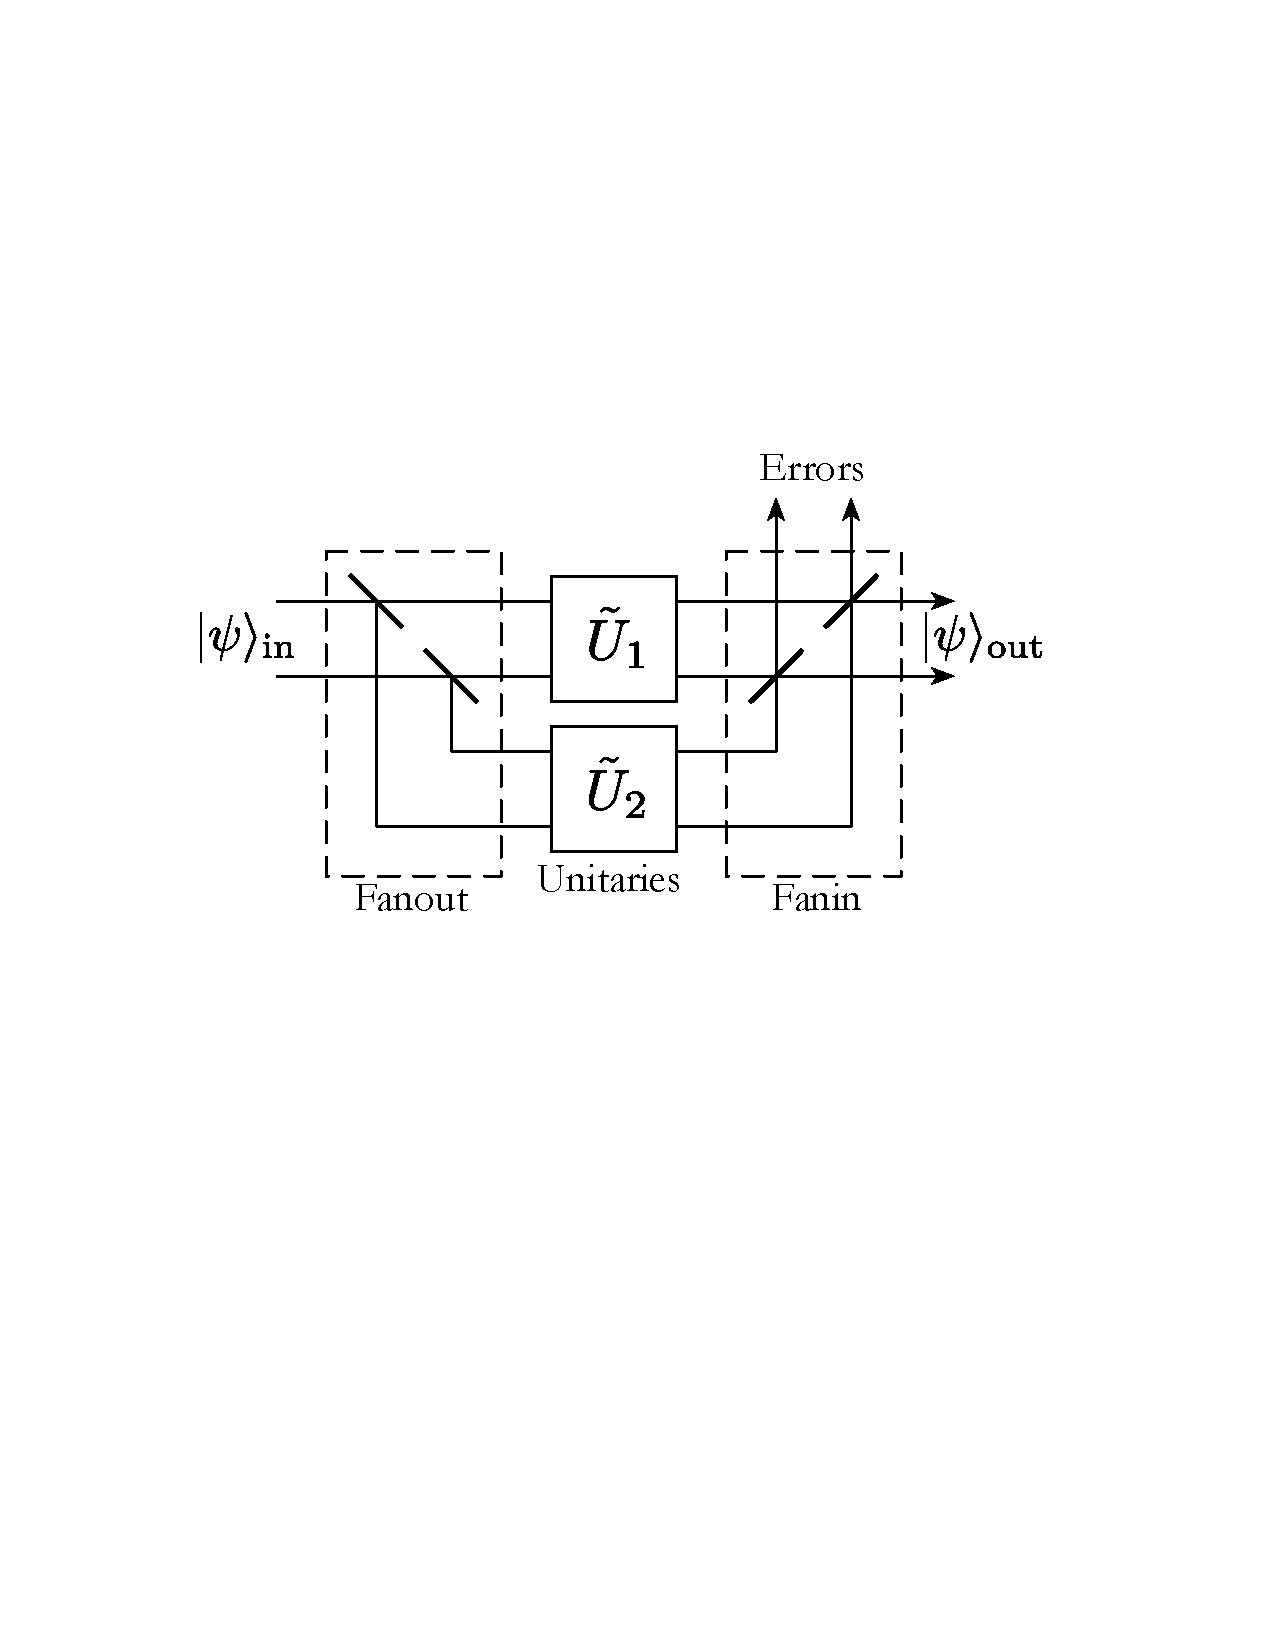
\includegraphics[clip=true, width=0.475\textwidth]{unitary_error_averaging}
\captionspacefig \caption{Protocol for error correction via unitary error averaging. Here our computation resides across \mbox{$N=2$} modes, and there are \mbox{$M=2$} redundant copies of the manufactured unitary, which straightforwardly generalises to arbitrary $M$ and $N$. A fanout operation splits the wave amplitudes from the set of $N$ input modes uniformly across $M$ sets of $N$ modes. Each set of $N$ evolves through an independent copy of the manufactured imperfect unitary, $\tilde{U}_i$. A reverse fanout operation recollects the bundles of modes. Upon post-selecting upon detecting all photons within the first $N$ modes, and none in the other ancillary modes, the state is projected into the subspace as if it had been acted upon by the arithmetic average of the imperfect unitaries. If photons are detected in the error modes, our logical state has effectively suffered photon loss and has been corrupted.} \label{fig:error_av_circuit}	
\end{figure}

Note that the protocol doesn't require that the $M$ instances of the unitary be held locally. They operate independently in parallel and could therefore be distributed, with the independent copies held by entirely different parties in distant locations (Sec.~\ref{sec:error_av_parallel}).\index{Distributed quantum computation}\index{Parallelisation}

The protocol is necessarily non-deterministic, since sometimes photons will be measured in the error modes, signalling that the output state has been projected onto an erroneous subspace. Thus, this is a heralded error correction scheme. When post-selection succeeds we have effectively evolved via the averaged operator, which statistically ought to more closely approximate $\hat{U}_\mathrm{target}$ than individual $\tilde{U}_i$.

%
% Qubit Loss Codes
%

\subsection{Qubit loss codes}\index{Qubit loss codes}

More severe than a simple, say, dephasing channel is qubit loss, whereby an entire physical qubit is lost to the environment, effectively tracing it out of the system. Depending on physical architecture, there are two ways in which qubit loss might manifest itself:
\begin{itemize}
\item Located errors\index{Located errors}: We know that a loss occurred and which physical qubit was affected.
\item Unlocated errors\index{Unlocated errors}: We do not know that a physical qubit was lost.
\end{itemize}

These manifestations arise naturally in different architectural contexts. For example, it is relatively easy to look at an atomic qubit to see whether it's still where it should be, whereas observing a photonic qubit typically requires destroying it, making the former vulnerable to located errors and the latter to unlocated errors.

It turns out that the distinction between these two modes of error can have a significant effect on the error correction thresholds of QECs. Specifically, a located error effectively gives us an additional classical bit of information diagnosing that an error took place, which we are not privy to for unlocated errors. This additional bit of information can be exploited by QEC codes to improve thresholds for located errors.

In \cite{RohdeHaselgrove} a derivation of a generalisation of the quantum Hamming bound\index{Quantum Hamming bound} for non-degenerate\footnote{In a non-degenerate code, all correctable errors map the codeword to orthogonal states. For degenerate codes\index{Degenerate codes} multiple distinct errors can map the codeword to the same state. The Hamming bound exploits the non-degeneracy using a counting or `pigeonholing' argument to count correctable errors.} QEC codes\index{Non-degenerate codes} was presented, where the number of located and unlocated errors were treated as independent parameters. They found that for non-degenerate codes the Hamming bound allows exactly twice as many located as unlocated errors. Specifically, for $t_l$ located errors and $t_u$ unlocated errors in an $n$-qubit non-degenerate code encoding $k$ logical qubits, QEC is possible provided that the number of errors satisfied,
\begin{align}
\sum_{i=0}^{t_u + \lfloor t_l/2 \rfloor} \binom{n}{i}3^i 2^k \leq 2^n.
\end{align}

Subsequently, using surface codes \cite{bib:StaceBarrettDohertyLoss} arrived at the similar conclusion that QEC codes are more robust against located than unlocated errors.

%
% Gate Failure Codes
%

\subsection{Gate failure codes}\index{Gate failure codes}

Quantum gates, especially 2-qubit entangling ones in many architectures, can have some non-zero chance of failure. In linear optics this gate non-determinism is an inherent feature of entangling gates like the CNOT. In fact it is provable that such gates cannot be implemented deterministically. With a large number of such gates in a circuit, the probability of them all working drops exponentially with the number of non-deterministic gates, thereby undermining efficiency. Can we overcome this?

In Sec.~\ref{sec:CS_LO} we discuss techniques for performing scalable linear optics quantum computing with non-deterministic gates, within the cluster state formalism\index{Cluster states}. The idea is to construct micro-clusters\index{Micro-cluster states} with redundant dangling bonds, which facilitate multiple bonding attempts to merge smaller clusters into larger ones. Once all the entangling operations have been performed, all that remains is to perform a sequence of single-qubit unitaries and measurements, both of which are deterministic in-principle.

This same approach could be logically generalised to any physical architecture where entangling gates are non-deterministic, but single-qubit operations are deterministic. 

%
% Decoherence-Free Subspaces
%

\subsection{Decoherence-free subspaces}\index{Decoherence-free subspaces}

The QoS techniques discussed previously were based on the notion of performing measurements on quantum systems to project them into subspaces devoid of errors. For example, in the 3-qubit code, measurement of the syndrome qubits projects the encoded state into a subspace where there was either no error, or in which an error occurred whose location is known and may therefore be corrected.

An alternate approach is to encode quantum information into Hilbert spaces which are invariant under a given error model. Such spaces are referred to as \textit{decoherence-free subspaces} (DFSs). In this instance we assume the error model is known, for example a dephasing channel, such that we can choose the appropriate DFS.

To illustrate this idea we will consider encoding a single logical qubit into two physical qubits. The error model we will encode against is a collective $Z$-rotation, where the two physical qubits are subject to perfectly correlated $Z$ errors. This arises naturally in the context of, say, atomic qubits subject to the same external electromagnetic field, and therefore accumulate the associated phase errors in tandem.

A single-qubit $Z$-rotation of angle $\theta$ on the Bloch sphere\index{Bloch sphere} is given by,
\begin{align}
	\hat{Z}(\theta) = e^{i\frac{\theta}{2}\hat{Z}} = \left(\begin{matrix}
  e^{i\frac{\theta}{2}} & 0 \\
  0 & e^{-i\frac{\theta}{2}}
\end{matrix}\right).
\end{align}
where $\hat{Z}$ is the usual Pauli phase-flip operator\index{Pauli operators} (Sec.~\ref{sec:circuit_model}). This operates on the physical basis states as,
\begin{align}
	\hat{Z}(\theta) \ket{0} &\to e^{i\frac{\theta}{2}}\ket{0}, \nonumber \\
	\hat{Z}(\theta) \ket{1} &\to e^{-i\frac{\theta}{2}}\ket{1}.
\end{align}

Now we employ the encoding for logical basis states,
\begin{align}
\ket{0}_L &\equiv \ket{0}_1\otimes\ket{1}_2,\nonumber \\
\ket{1}_L &\equiv \ket{1}_1\otimes\ket{0}_2,
\end{align}
Note that both logical basis states are invariant under a common $Z$-rotation (the other two physical basis states, $\ket{0}_1\otimes\ket{0}_2$ and $\ket{1}_1\otimes\ket{1}_2$ do not observe this property),
\begin{align}
	\hat{Z}_1(\theta)\hat{Z}_2(\theta)\ket{0}_L &= \ket{0}_L,\nonumber\\
	\hat{Z}_1(\theta)\hat{Z}_2(\theta)\ket{1}_L &= \ket{1}_L.
\end{align}
Thus, when acting on an arbitrary linear combination of these basis states (i.e a logical qubit),
\begin{align}
\ket\psi_L = \alpha \ket{0}_L + \beta\ket{1}_L,
\end{align}
via linearity the logical qubit must also be invariant under the collective error,
\begin{align}
	\hat{Z}_1(\theta)\hat{Z}_2(\theta)\ket\psi_L = \ket\psi_L.
\end{align}
This type of DFS encoding therefore protects a logical qubit against arbitrary, unknown but correlated $Z$-rotations.

The same principle can be logically extended to many other correlated error models. For example, operating in a rotated basis (under a Hadamard transform), one could similarly protect against correlated $X$-rotations using the encoding,
\begin{align}
\ket{0}_L &\equiv \ket{-}_1\otimes\ket{+}_2,\nonumber \\
\ket{1}_L &\equiv \ket{+}_1\otimes\ket{-}_2,
\end{align}
where \mbox{$\ket\pm=\frac{1}{\sqrt{2}}(\ket{0}\pm\ket{1})$}.

This idea, although very simple, is very powerful, since it is a completely passive form of error correction, requiring no syndrome measurements, feedforward or correction operations. It also arises quite naturally in some systems where undesired external fields act roughly uniformly across the physical qubits within a system.

%
% Dynamical Decoupling
%

\subsection{Dynamical decoupling}\index{Dynamical decoupling}

An alternate mechanism by which errors could be introduced into our system is via coupling to an external environment (for example via an electromagnetic field) introducing a persistent evolution of our qubits, which is slow-moving compared to the rate at which the implemented computation is evolving the system. We can model this as a joint system/environment Hamiltonian of the form,
\begin{align}\label{eq:dyn_dec_ham}
\hat{H}_\mathrm{total} = \lambda_\mathrm{comp}\hat{H}_\mathrm{comp} + \lambda_\mathrm{env}\hat{H}_\mathrm{env} + \lambda_\mathrm{int}\hat{H}_\mathrm{int},	
\end{align}
where the different components represent, in order, the Hamiltonians of the: total joint system; quantum computer (or system of interest); environment; interaction between system and environment. We are specifically operating in the regime where \mbox{$\lambda_\mathrm{int}\ll\lambda_\mathrm{comp}$}, such that the computation is the dominant term in the evolution and the environmental coupling can be treated as a small perturbation from the desired evolution.

The goal of dynamical decoupling is to minimise the influence of the system/environment interaction term, $\hat{H}_\mathrm{int}$, by manipulating the system in such a way that this term continuously cancels itself out over time.

Let us illustrate how this can be achieved using a simple example, whereby a single-qubit system couples with an environment which introduces a slow, unknown phase evolution. Discretising time, we can write this phase evolution as a Pauli $Z$-rotation on the Bloch sphere\index{Bloch sphere},
\begin{align}
	\hat{Z}(\theta) = e^{i\frac{\theta}{2}\hat{Z}} = \left(\begin{matrix}
  e^{i\frac{\theta}{2}} & 0 \\
  0 & e^{-i\frac{\theta}{2}}
\end{matrix}\right),
\end{align}
for some unknown, but small $\theta$. Next we observe that, quite obviously, a $Z$-rotation of angle $\theta$ can be trivially undone by applying another $Z$-rotation of angle $-\theta$, since,
\begin{align}
\hat{Z}(-\theta)\hat{Z}(\theta) = \hat{\mathbb{I}}.	
\end{align}

Therefore, if the system/environment coupling introduced an evolution of $\hat{Z}(\theta)$ in the previous unit of time, our goal is to manipulate it into implementing $\hat{Z}(-\theta)$ during the next one. Alas, the environment is beyond our control and we cannot directly order it to reverse direction. We do, however, have complete control over our qubit system, so we will achieve the same outcome by flipping the direction of the Bloch sphere underneath the environments foot, allow it to take a step forward, before flipping it back.

How do we achieve this flip in the Bloch sphere? Simply by using the following identity from the algebra of the Pauli matrices\index{Pauli operators},
\begin{align}
\hat{X}\hat{Z}(\theta)\hat{X} = 	\hat{Z}(-\theta).
\end{align}
That is, applying a bit-flip to a qubit, followed by an arbitrary phase-rotation, followed by another bit-flip is equivalent to having taken the same phase-rotation in the reverse direction. Effectively we are tricking the environment into time-reversal!

Now if we proceed for two time-steps, once bit-flipped and another not, we have,
\begin{align}
\underbrace{\hat{Z}(\theta)}_{\mathrm{forward}}\cdot\underbrace{[\hat{X}\hat{Z}(\theta)\hat{X}]}_{\mathrm{reverse}} = \hat{\mathbb{I}},
\end{align}
and the unknown phase-rotation has been eliminated. The sequence is illustrated on the Bloch sphere\index{Bloch sphere} in Fig.~\ref{fig:bloch_sphere_dyn_dec}.

\if 2\pubmode
	\begin{figure}[!htbp]
	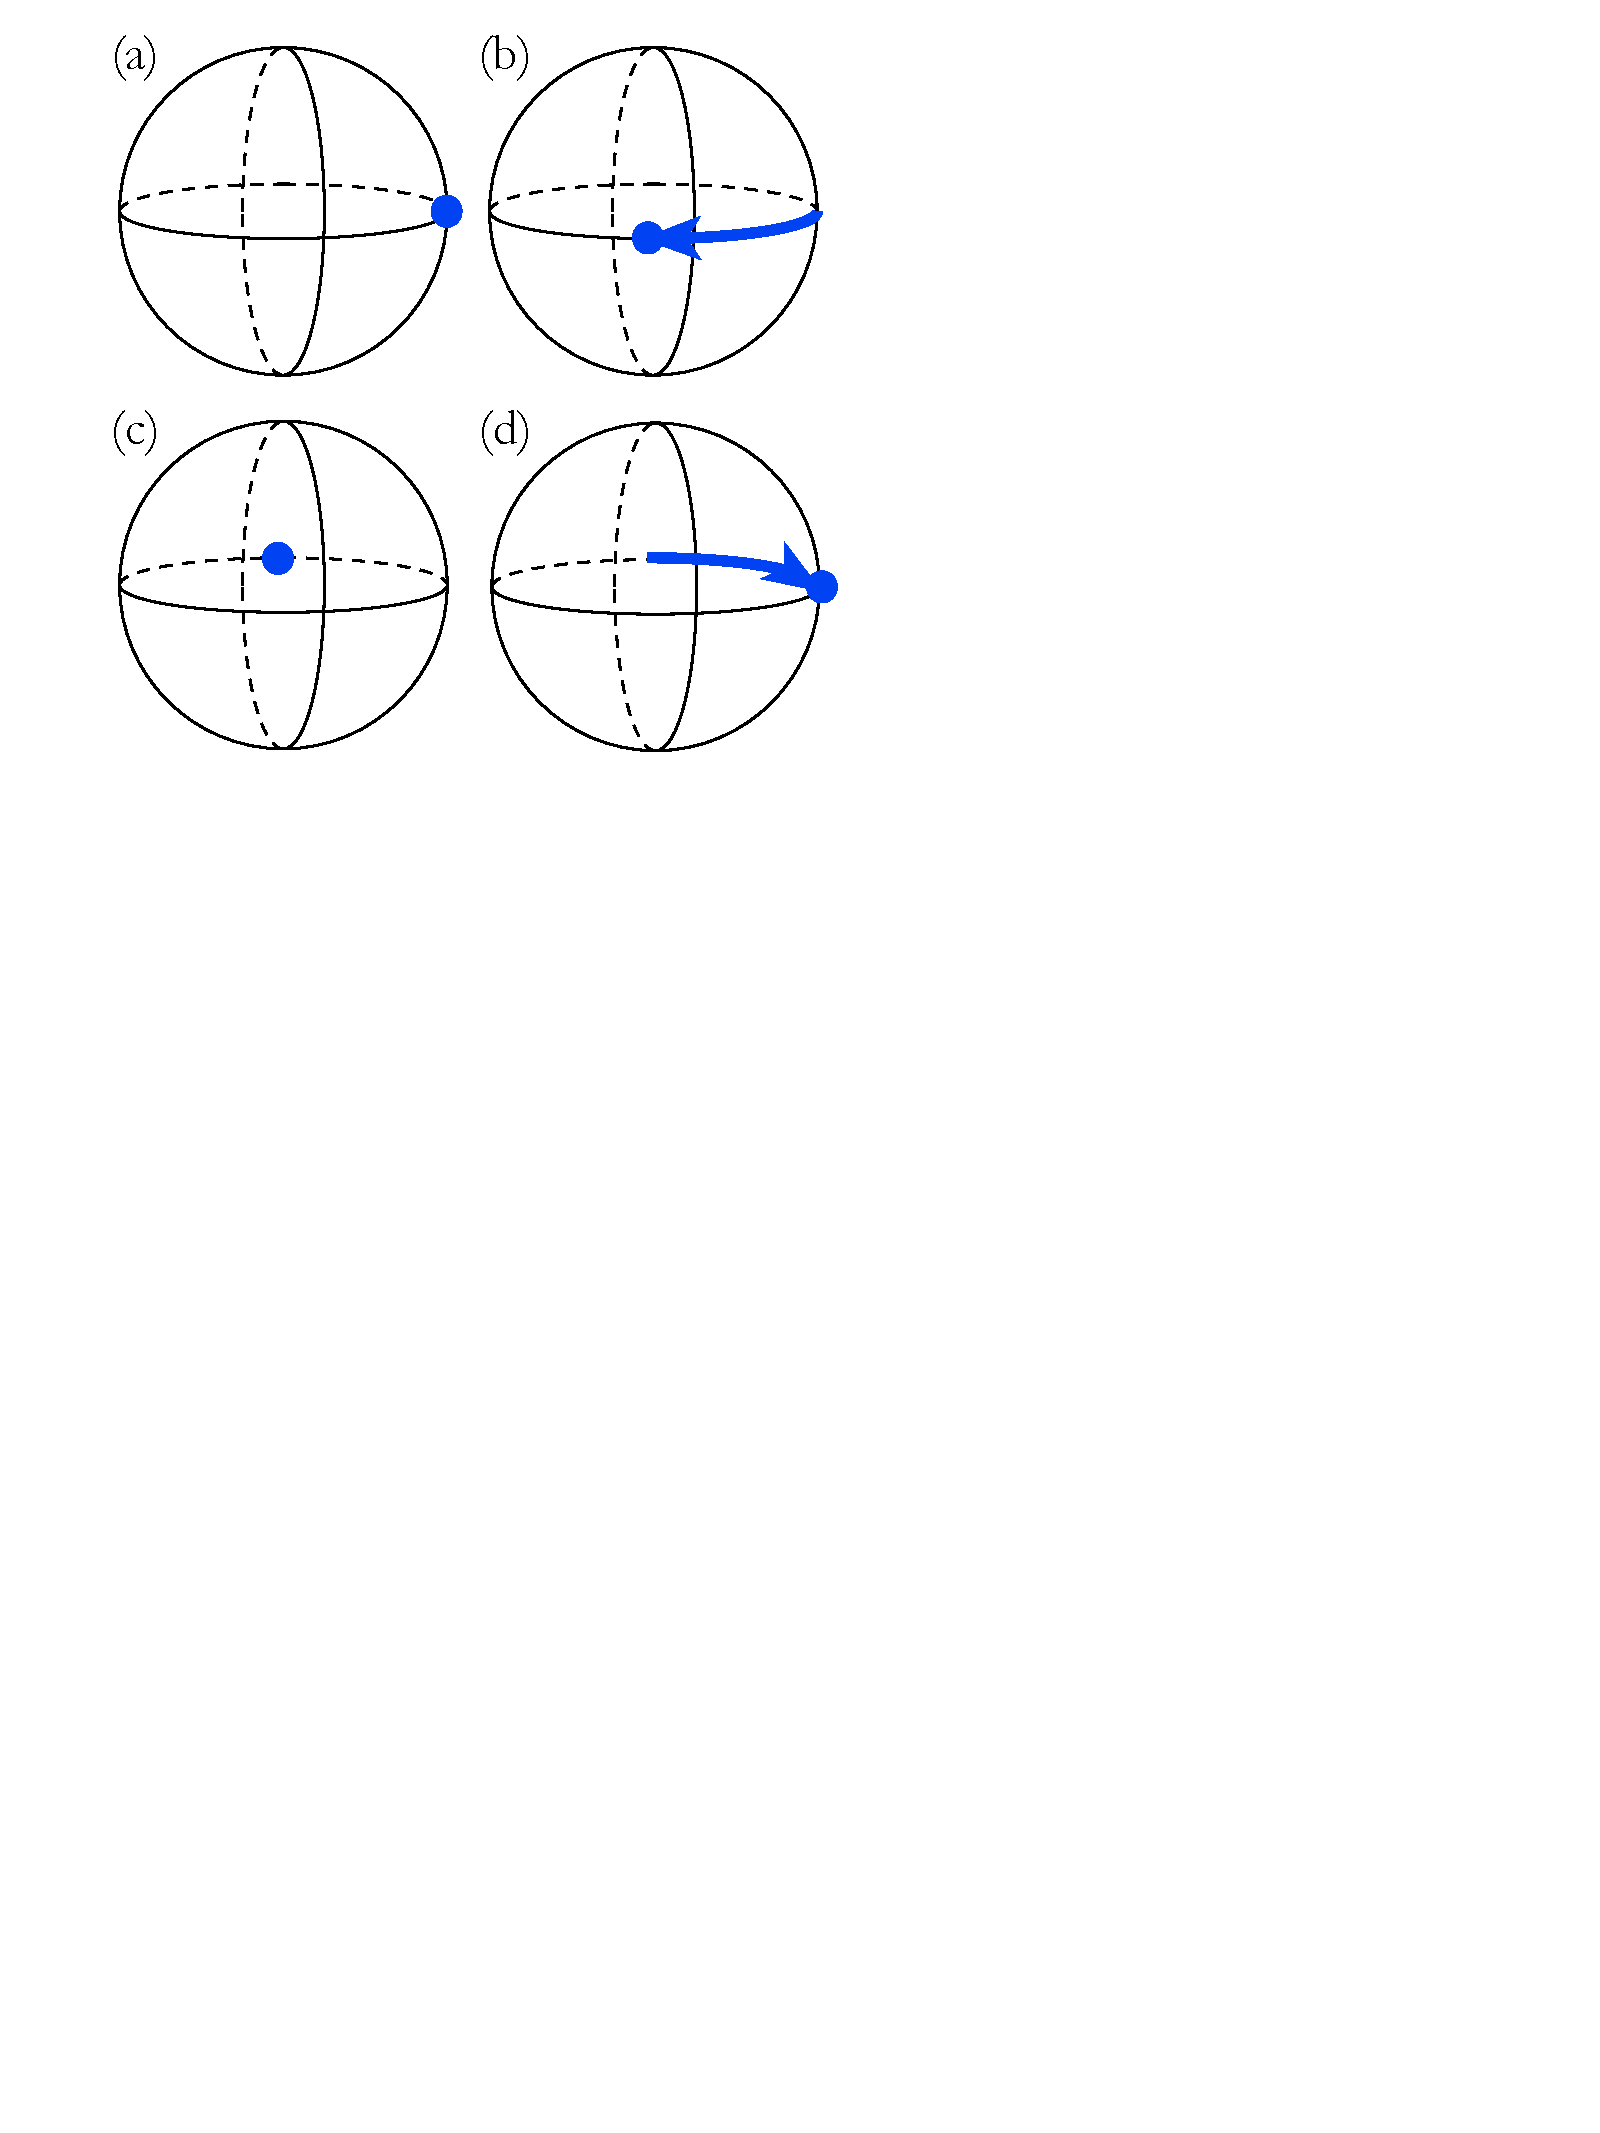
\includegraphics[clip=true, width=0.475\textwidth]{bloch_sphere_dyn_dec_long}
	\captionspacefig \caption{Bloch sphere representation of a sequence to dynamically decouple an unknown $\hat{Z}$ rotation from a qubit. (a) Blue dot represents the initial state. (b) The state undergoes an unknown $\hat{Z}(\theta)$ rotation. (c) A bit-flip ($\hat{X}$) flips the Bloch sphere upside down. (d) Waiting for the same time as before such that the same unknown $\hat{Z}$-rotation takes place, the state ends up in its initial state, independent of the $\hat{Z}$-rotation angle $\theta$, but assuming it was the same on both occasions in (b) and (d).} \label{fig:bloch_sphere_dyn_dec}	
	\end{figure}
\else
	\begin{figure*}[!htbp]
	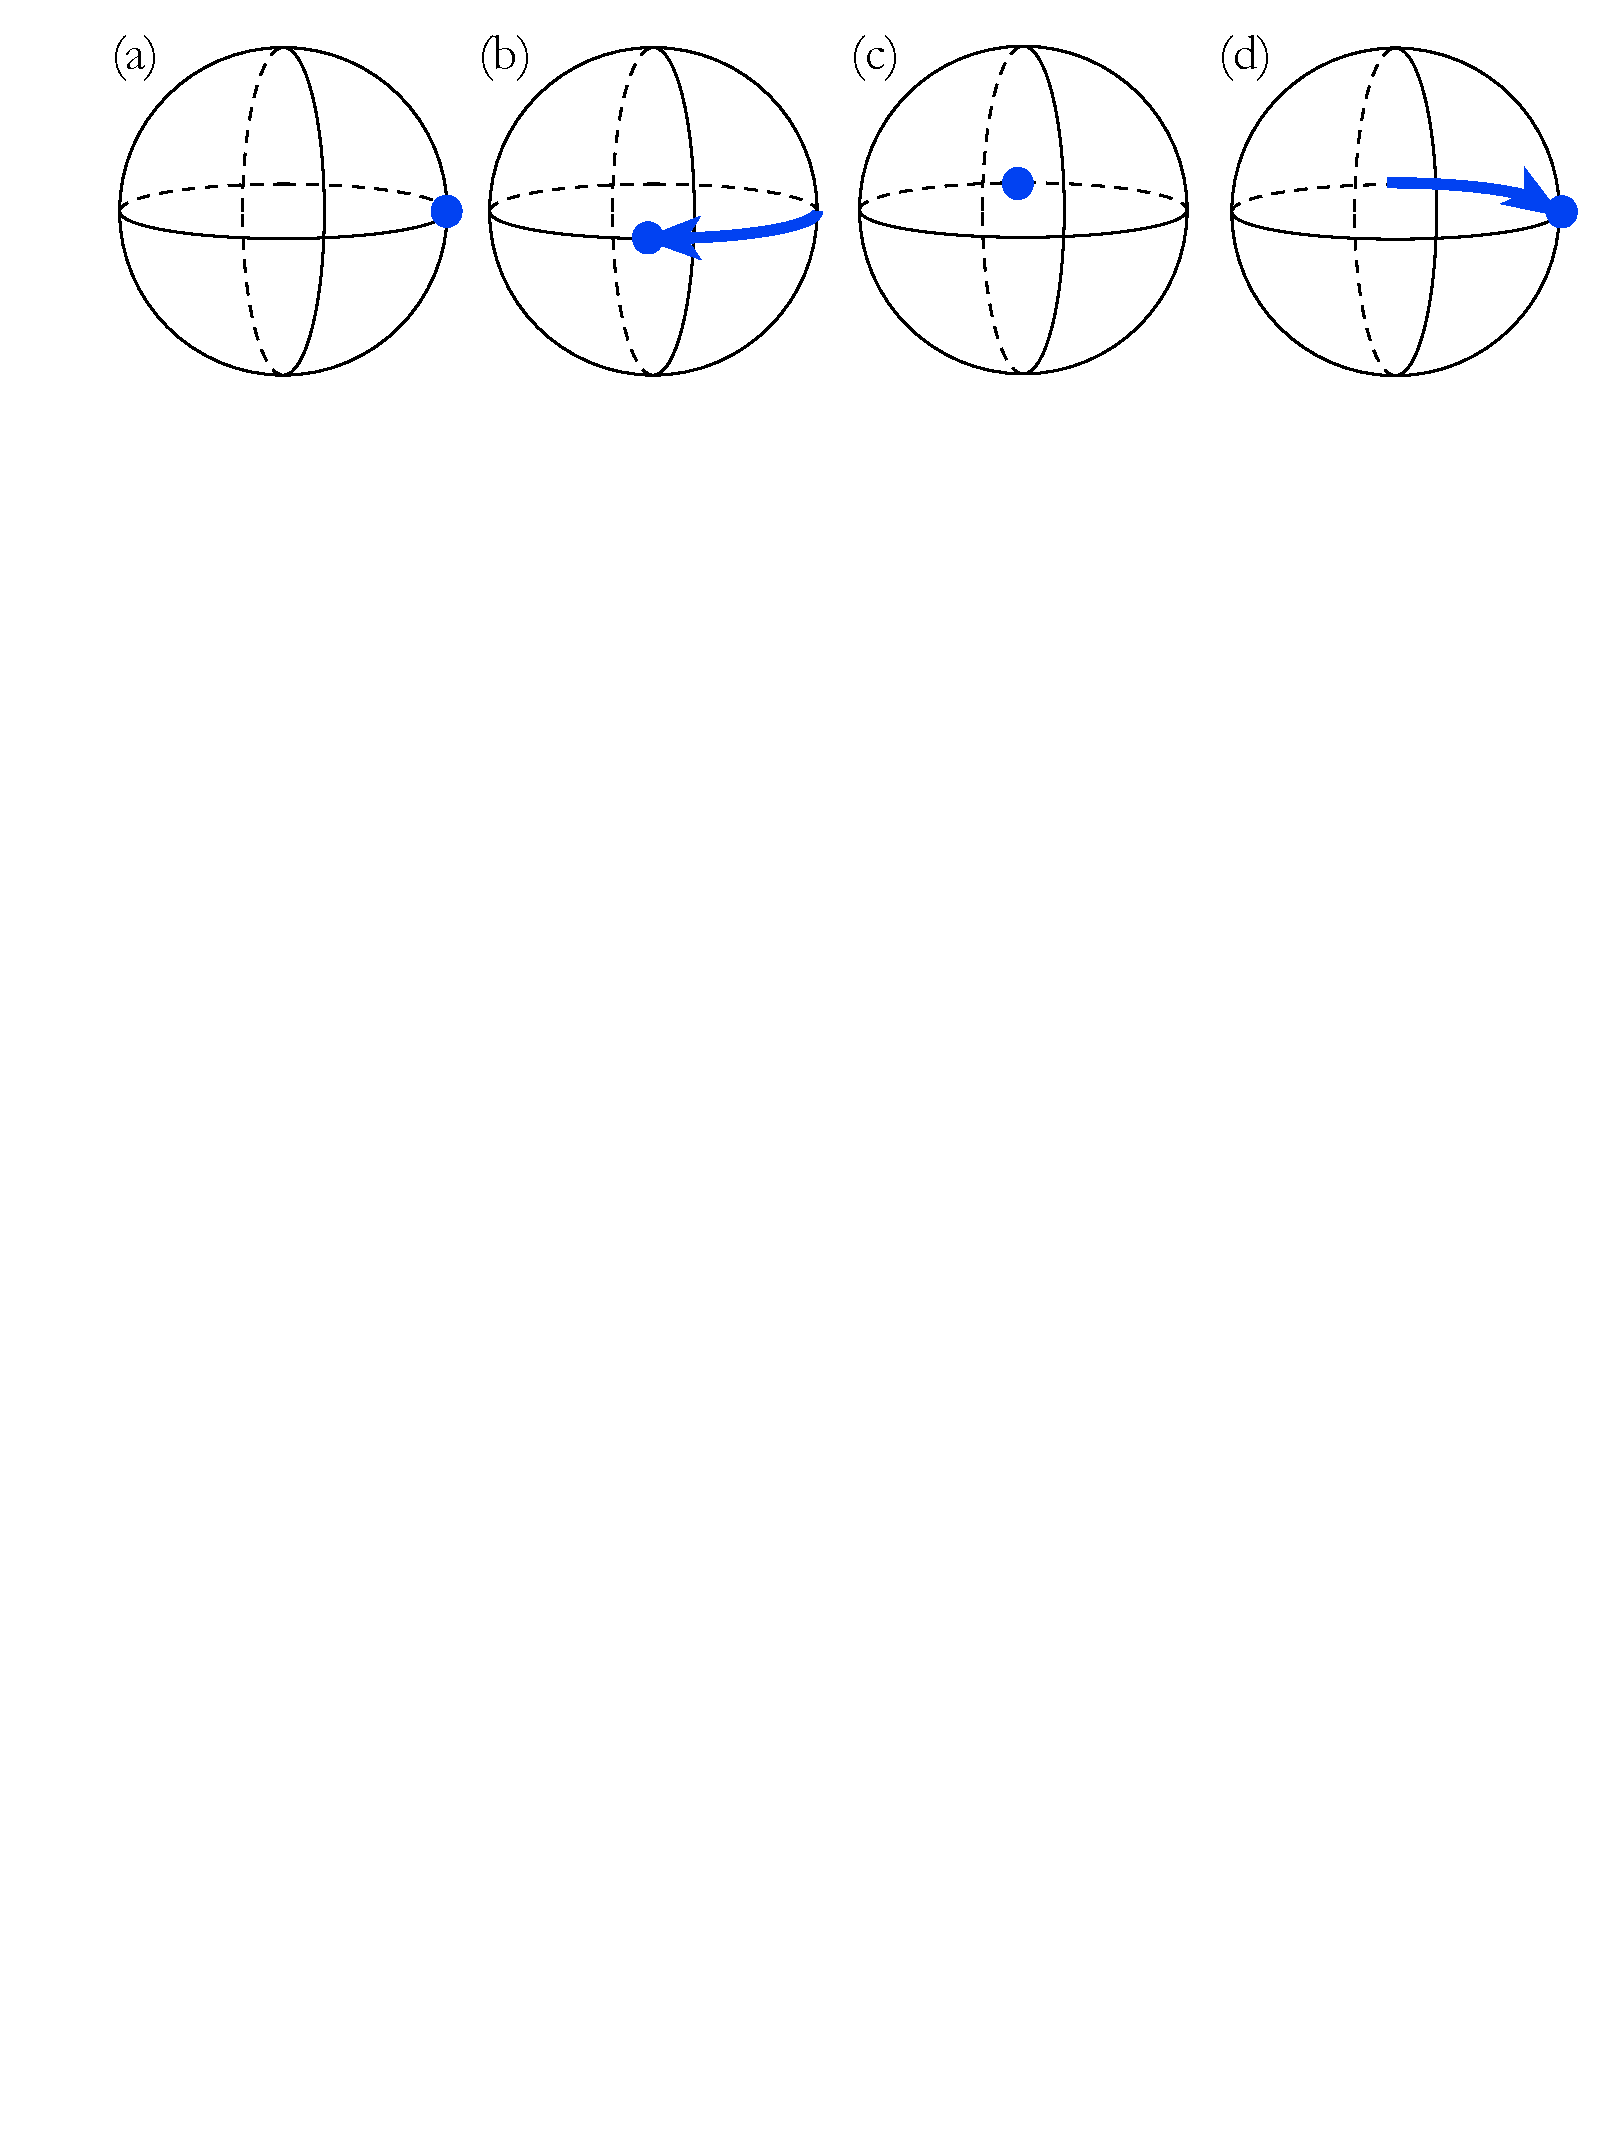
\includegraphics[clip=true, width=\textwidth]{bloch_sphere_dyn_dec}
	\captionspacefig \caption{Bloch sphere representation of a sequence to dynamically decouple an unknown $\hat{Z}$ rotation from a qubit. (a) Blue dot represents the initial state. (b) The state undergoes an unknown $\hat{Z}(\theta)$ rotation. (c) A bit-flip ($\hat{X}$) flips the Bloch sphere upside down. (d) Waiting for the same time as before such that the same unknown $\hat{Z}$-rotation takes place, the state ends up in its initial state, independent of the $\hat{Z}$-rotation angle $\theta$, but assuming it was the same on both occasions in (b) and (d).} \label{fig:bloch_sphere_dyn_dec}	
	\end{figure*}
\fi

The coupling to the external environment and the qubit state needn't be constant over time, but could be time-varying. In this instance, it is essential that the decoupling control sequence of bit-flip operations be much faster than the rate at which both the phase-rotations and computational operation are changing, such that consecutive unknown phase-rotations are approximately equal and thereby almost perfectly cancel. This rapid control sequence is sometimes referred to as `bang-bang' control\index{Bang-bang control}, since we are repeatedly implementing bit-flips at a fast rate. 

As described above, we have merely error corrected a quantum memory. Of course we wish to implement far more sophisticated evolutions. This requires breaking down the computational evolution (given by $\hat{H}_\mathrm{comp}$) into a large number of small, discrete steps. These are interspersed with our bang-bang control sequence so as to continuously remove any phase-errors accumulated during the course of the computation.

Dynamical decoupling extends to all manner of error models, beyond the simple $Z$-error model presented above. They are therefore a very powerful tool in error correction. However, unfortunately they are only naturally suited to continuous evolutions governed by Hamiltonians of the form shown in Eq.~(\ref{eq:dyn_dec_ham}), not to the more common discretised models such as the circuit and cluster state models.

\comment{References}

%
% Continuous-Variables
%

\subsection{Continuous-variables}\index{Continuous-variable quantum error correction}

First CV QEC protocol is the direct analogue of the the qubit redundancy codes. However, the noise models do not correspond to what usually occur in Gaussian systems, namely, thermal noise\index{Thermal noise} and loss.

It has been proven that QEC of Gaussian noise on Gaussian states, using only Gaussian operations is impossible \cite{bib:PhysRevLett.102.120501}. It is closely related to entanglement distillation, discusses above. Several approaches have since been developed. One proposes to encode information in non-Gaussian CV states, then error correction can be implemented using Gaussian operations, resulting in a Gaussian state \cite{bib:pirandola2004constructing}. Another approach is to error correct on Gaussian states using non-Gaussian operations, similar to the entanglement distillation protocol. It is unclear which one is the most advantageous.

\comment{To do -- can we be a bit more specific about the physical resource requirements and the specific noise models? Specify what Gaussian noise means.}